% Standalone draft project: Methodology + Experimental Results chapters only.
% Extracted from the full thesis template so these two chapters can be
% iterated on in isolation, without the title page, abstract, or
% introduction/preliminaries chapters. Once finalized, copy the content back
% into 3-methodology.tex / 4-results.tex in the main thesis project.

\documentclass[12pt, a4paper]{report}

\usepackage{fontspec}
\usepackage{polyglossia}
\setdefaultlanguage{english}

\usepackage{csquotes}

\usepackage[
    maxbibnames=50,
    sorting=nty
]{biblatex}
\addbibresource{bibliography.bib}

\usepackage{setspace}
\onehalfspacing

\usepackage{geometry}
\geometry{margin=2.5cm}

\usepackage{graphicx}
\graphicspath{
    {../Thesis_template__Faculty_of_Mathematics_and_Informatics__University_of_Bucharest__1_/images/}
    {../../data/graphs/EDA/credit_card/}
    {../../data/graphs/EDA/yahoo/}
    {../../data/graphs/EDA/cicids/}
}

\usepackage{booktabs}
\usepackage{listings}
\usepackage{float}

\usepackage[
    colorlinks,
    linkcolor={black},
    menucolor={black},
    citecolor={black},
    urlcolor={blue}
]{hyperref}

\usepackage[warnings-off={mathtools-colon,mathtools-overbracket}]{unicode-math}
\usepackage{amsmath}
\usepackage{mathtools}

\newcommand{\bigO}[1]{\symcal{O}\left(#1\right)}
\DeclarePairedDelimiter\abs{\lvert}{\rvert}

\begin{document}

\tableofcontents

\chapter{Methods and Experimental Setup}
\label{ch:methodology}

% This chapter explains every model and every shared experimental choice
% (preprocessing, hyperparameters, evaluation protocol) that applies across
% all three datasets. Dataset-specific preprocessing details that don't
% generalize (e.g. exact feature counts, window lengths) can either stay
% here at a high level or move into the per-dataset Results subsections --
% decide per case once the prose is drafted.

\section{Research Design and Approach}
\label{sec:approach}

This project is organized around a single question: how does the way a model represents the \emph{latent structure} of "normal" data determine what kinds of anomalies it can and cannot detect? Rather than optimizing one architecture for one dataset, the approach taken here is deliberately comparative along two axes at once.

The first axis is \textbf{paradigm}: the seven models evaluated (\S\ref{sec:algorithms}) were chosen specifically to cover four structurally distinct ways of representing what "normal" looks like -- a \textbf{boundary} carved out in kernel space (One-Class SVM), a \textbf{partitioning} of the feature space by random splits (Isolation Forest), a learned \textbf{compression bottleneck} that must discard everything but the dominant structure of normal data (the three reconstruction-based autoencoders), and a \textbf{predictive} model of how normal data evolves one step at a time (Predictive LSTM, Causal Transformer). These are not arbitrary choices or a convenience sample of popular architectures: each paradigm encodes a different implicit assumption about what makes a point anomalous, and the central empirical question throughout this thesis is which assumption matches which kind of anomaly.

The second axis is \textbf{dataset}: Credit Card Fraud, Yahoo Webscope S5, and CIC-IDS2017 (\S\ref{sec:datasets}) were selected to span a deliberate spectrum of temporal structure -- from a purely tabular dataset with no meaningful ordering between rows, through genuinely sequential time series, to network flow data that admits flat, temporal, and host-context views of the same underlying events. Running every model paradigm against every point on this spectrum is what makes it possible to attribute a given result to the \emph{paradigm} (does this kind of anomaly need a predictive objective, or a bottleneck, or neither?) rather than to some idiosyncrasy of a single dataset.

The resulting experimental method follows a fixed three-stage cycle, repeated per dataset in Chapter~\ref{ch:results}:

\begin{enumerate}
  \item \textbf{Measure.} Train every applicable model exclusively on benign data and evaluate all of them under the same protocol (\S\ref{sec:eval-protocol}), producing a ranked comparison table and, where the data supports it, a breakdown by anomaly type or attack class.
  \item \textbf{Explain.} Read the resulting performance gaps -- not just which model wins, but which paradigm wins where -- and propose a concrete mechanistic explanation grounded in each model's architecture (e.g.\ "the LSTM Autoencoder's pooled hidden state destroys the phase information a seasonal anomaly needs").
  \item \textbf{Verify.} Treat that explanation as a falsifiable claim and test it directly with a targeted diagnostic -- reconstruction-error localization, SHAP attribution, or a controlled perturbation of the input -- rather than letting the aggregate metrics alone stand as evidence for the mechanism. Chapter~\ref{ch:explainability} is dedicated entirely to this stage, and its findings are reported honestly as confirming, complicating, or refining the claims made in Chapter~\ref{ch:results}, not merely as illustrations of them.
\end{enumerate}

This cycle is what separates the thesis's contribution from a plain benchmark comparison: the goal is not only to report which of seven models scores highest on which of three datasets, but to build and test an explanation of \emph{why}, at the level of paradigm rather than individual model.

\section{Anomaly Detection Algorithms}
\label{sec:algorithms}

All models below are used for \emph{novelty detection}, not outlier detection: each is fit exclusively on benign/normal data and never sees an anomaly during training, so "normal" is whatever the training distribution looked like. At test time each model produces a scalar anomaly score per sample (never a hard label directly), and the label is obtained by thresholding that score with the procedure in \S\ref{sec:eval-protocol}. The seven models fall into four paradigms: \textbf{boundary-based} (One-Class SVM), \textbf{partition-based} (Isolation Forest), \textbf{reconstruction-based} (Feedforward Autoencoder, LSTM Autoencoder, Bottleneck Transformer Autoencoder), and \textbf{temporal-predictive} (Predictive LSTM, Causal Transformer).

\subsection{One-Class SVM}

One-Class SVM (\texttt{sklearn.svm.OneClassSVM}, $\nu$-SVM formulation) learns a boundary around the training data in a (typically infinite-dimensional) feature space induced by a kernel, rather than reconstructing or partitioning the input directly. With the RBF kernel used throughout this project, the model implicitly fits a smooth, closed decision region around the bulk of the benign training points. Fixed across all three datasets: \texttt{kernel='rbf'}, \texttt{nu=0.01}, \texttt{gamma='scale'} (see \S\ref{sec:architecture}). At test time, \texttt{decision\_function} returns the signed distance to the learned boundary (positive inside, negative outside); this is negated so that, consistently with every other model in this project, \emph{higher score = more anomalous}.

\subsection{Isolation Forest}

Isolation Forest (\texttt{sklearn.ensemble.IsolationForest}) is partition-based: it builds an ensemble of random trees that recursively split the feature space on randomly chosen features and split points, and uses the average path length required to isolate a point (into its own leaf) across all trees as the anomaly signal. Because splits are random, points that are easy to separate from the rest of the data -- i.e.\ anomalies, which tend to sit in sparse, low-density regions -- are isolated in fewer splits, giving them a shorter average path length than typical benign points. \texttt{score\_samples} returns the negative mean path length, which is negated once more here so that higher score means shorter path (i.e.\ more anomalous), keeping the convention consistent with every other model. \texttt{contamination} is left at its default, \texttt{'auto'}: this parameter would normally set the model's own internal decision threshold based on an assumed anomaly fraction in the training data, but since training data here is exclusively benign (no contamination to speak of) and the operating threshold is instead selected externally via the PR-curve sweep in \S\ref{sec:eval-protocol}, \texttt{contamination} has no effect on the reported results -- only the continuous anomaly score matters.

\subsection{Feedforward (MLP) Autoencoder}

The Feedforward Autoencoder is reconstruction-based: a symmetric encoder/decoder pair of fully-connected \texttt{Linear}+\texttt{ReLU} layers (with dropout between hidden layers) compresses the input feature vector down through a bottleneck of strictly reduced dimensionality and then expands it back to the original input size, trained end-to-end to minimize mean squared reconstruction error against its own input. Because the bottleneck is narrower than the input, the network cannot simply learn the identity function; it is forced to learn a compressed representation that captures the dominant structure of \emph{benign} data specifically. At test time, the anomaly score is the per-sample mean squared error between the input and its reconstruction: benign samples, which resemble the training distribution the bottleneck was shaped around, reconstruct with low error, while anomalous samples -- which the bottleneck was never trained to represent -- tend to reconstruct poorly. Layer widths and the resulting bottleneck ratio vary by dataset (\S\ref{sec:architecture}) but the encoder/decoder-mirror-of-encoder architecture is identical everywhere.

\subsection{LSTM Autoencoder}

The LSTM Autoencoder applies the same reconstruction principle as the Feedforward Autoencoder, but to sequence-shaped input: one LSTM layer serves as the encoder, consuming the full input sequence and retaining only its final hidden (and cell) state as a single fixed-size vector summary of the entire sequence. That final hidden state is then repeated identically at every timestep as the input to a second LSTM layer acting as the decoder, whose per-timestep outputs are projected back to the original feature dimensionality by a shared linear layer. The anomaly score is again per-sample mean squared error, computed over every timestep and feature jointly between the input sequence and its reconstruction.

\subsection{Predictive LSTM}

The Predictive LSTM uses the same recurrent building block (a single LSTM layer) as the LSTM Autoencoder above, but with a categorically different training objective: rather than reconstructing its own input, it is trained to predict step $t+1$ from steps $0..t$ at every position in the sequence simultaneously -- the model never sees the value it is being asked to predict. Architecturally, this means the LSTM's hidden state at each timestep is projected directly to a next-step prediction via a linear output layer, with no encoder/decoder split and no bottleneck vector: the model consumes the sequence once, and every hidden state along the way is used, rather than only the final one. The anomaly score is the mean squared error between predicted and true next-step values across the sequence. This distinction in \emph{objective} (predict the future vs.\ reconstruct the present), rather than any difference in raw architectural capacity, is what separates this model from the LSTM Autoencoder, and turns out to matter substantially more than the choice of recurrent vs.\ attention-based backbone for how each model responds to different anomaly types (\S\ref{ch:results}).

\subsection{Transformer-Based Autoencoders}

Two transformer variants are used, both replacing the LSTM Autoencoder's recurrent backbone with a multi-layer \texttt{TransformerEncoder} (self-attention + feedforward blocks, sinusoidal positional encoding, identical \texttt{D\_MODEL}/\texttt{NHEAD}/\texttt{NUM\_LAYERS}/\texttt{DIM\_FF} across datasets -- \S\ref{sec:architecture}), but differing in how the bottleneck (reconstruction) or causality (prediction) constraint is imposed:

\begin{itemize}
  \item \textbf{Bottleneck Transformer Autoencoder} -- reconstruction-based. Each input feature/timestep is projected to a $\texttt{D\_MODEL}$-dimensional token and passed through the transformer encoder with full (non-causal) self-attention, so every position can attend to every other position freely. The resulting per-position representations are then \emph{global-average-pooled} across the sequence into a single $\texttt{D\_MODEL}$-dimensional vector, squeezed through a linear layer to a strictly smaller \texttt{LATENT\_DIM}, and expanded back out by a second linear layer to the full flattened sequence shape. This pool-squeeze-expand step is the explicit information bottleneck (analogous to the LSTM Autoencoder's final hidden state) that prevents the attention mechanism from simply copying its input through to the output. Anomaly score: per-sample MSE between input and reconstruction across all positions, computed in a single forward pass.
  \item \textbf{Causal Transformer} -- temporal-predictive, the attention-based counterpart to the Predictive LSTM. The same encoder stack is used, but with a causal (upper-triangular) attention mask applied, so position $t$ can only attend to positions $0..t$; the model is trained on the same next-step objective as the Predictive LSTM, with no pooling bottleneck. Anomaly score: per-sample MSE between predicted and true next-step values.
\end{itemize}

Both variants deliberately use a single \texttt{TransformerEncoder} stack rather than the full encoder-decoder structure common in the time-series transformer literature (e.g.\ Informer's ProbSparse-attention encoder paired with a generative decoder, or reconstruction-based designs that pair a Transformer encoder with a separate convolutional decoder). Training and inference cost scale with the number of attention layers on both datasets and models, and an encoder-only design keeps that cost, along with the number of trainable parameters, to roughly half of what an equivalent encoder-decoder model would require, without sacrificing the ability to either pool-and-reconstruct or causally predict.

No Causal Transformer implementation exists for the credit card dataset (\S\ref{ch:results}).

\section{Datasets}
\label{sec:datasets}

Three datasets were selected to span a deliberate spectrum of temporal structure: Dataset A is purely tabular, with no meaningful temporal ordering between rows; Datasets B and C are genuinely temporal, with Dataset C additionally admitting both a flat/tabular and a temporal view of the same underlying data. This lets the same four modeling paradigms be evaluated under progressively harder conditions for the "does temporal order matter" question.

\subsection{Credit Card Fraud Detection (Dataset A)}

The Kaggle Credit Card Fraud Detection dataset contains 284{,}807 transactions, of which 492 (0.172\%) are fraudulent -- an extreme class imbalance typical of real-world fraud detection. Each row has 30 features: \texttt{Time} (seconds elapsed since the first transaction in the dataset), 28 PCA-transformed features \texttt{V1}--\texttt{V28} (anonymized for confidentiality, already decorrelated and roughly zero-mean by construction), and \texttt{Amount} (raw transaction value, heavily right-skewed).

The dataset, along with community exploratory analysis, is available on Kaggle.\footnote{\url{https://www.kaggle.com/datasets/mlg-ulb/creditcardfraud}} A further exploratory notebook specifically covering imbalanced-data handling and anomaly detection on this dataset is also available.\footnote{\url{https://www.kaggle.com/code/janiobachmann/credit-fraud-dealing-with-imbalanced-datasets}}

\texttt{Time} is elapsed seconds, not a repeating or structured temporal axis -- there is no periodicity, trend, or session concept to exploit. This makes Dataset A the deliberate "no genuine temporal order" control case.

\subsection{Yahoo Webscope S5 (Dataset B)}

Yahoo Webscope S5 consists of four benchmark families (A1--A4), each a collection of independent univariate time series with labeled anomalies, but each constructed to isolate a different anomaly type:

\begin{center}
\resizebox{\textwidth}{!}{%
\begin{tabular}{@{}lllll@{}}
\toprule
Benchmark & Series & Origin & Anomaly type & Anomaly rate \\
\midrule
A1 & 67  & Real server metrics & Point outliers & 1.76\% \\
A2 & 100 & Synthetic, single periodic component + trend & Point outliers & 0.33\% \\
A3 & 100 & Synthetic, 3 interacting frequency components & Contextual (phase deviation) & 0.56\% \\
A4 & 100 & Synthetic, same structure, no seasonality & Level shifts & 0.50\% \\
\bottomrule
\end{tabular}%
}
\end{center}

A1 is real, organic, and noisy (messy daily/weekly cycles); A2--A4 are synthetic and purpose-built so that the anomaly type is controlled independently of the underlying series shape. This is what allows the Results chapter to attribute performance differences to \emph{anomaly type} (point vs.\ contextual vs.\ level-shift) rather than to confounding differences between datasets. A2 is included in the codebase but has only a partial run so far (see \S\ref{ch:results}).

\subsection{CIC-IDS2017 (Dataset C)}

CIC-IDS2017 (Canadian Institute for Cybersecurity) is a network intrusion detection benchmark captured over five working days: $\sim$2.8 million bidirectional network flows, each described by $\sim$80 statistical features extracted by CICFlowMeter (duration, packet/byte counts and rates, inter-arrival-time statistics, TCP flag counts, window sizes, etc.). Monday is 100\% benign traffic; 14 distinct attack types (DoS/DDoS variants, PortScan, brute-force, web attacks, Bot, Infiltration, Heartbleed) are injected Tuesday through Friday. The Monday-benign / rest-mixed split is therefore a natural, dataset-native novelty detection split.

The raw/Kaggle distribution of this dataset is known to be substantially corrupted (Engelen et al., WTMC 2021): roughly 26\% of flows are TCP "appendix" artifacts inheriting their parent flow's attack label without containing any attack traffic, a large fraction of nominally-labeled attack flows carry no actual payload (label-only, not behavior-based), and the entire \texttt{DoS Hulk} class corresponds to a broken attack simulation that never executes against the target server. Identifier columns (\texttt{Flow ID}, source/destination IP, \texttt{Timestamp}) are also present and, if kept, let a model shortcut-learn by IP address or capture time window instead of by traffic behavior. This project uses the cleaned, re-extracted version of the dataset from Engelen et al. rather than the original Kaggle/UNB CSVs, and drops the identifier columns explicitly (see \S\ref{sec:preprocessing}).

CIC-IDS2017 flows are session-level statistical aggregates. This makes the dataset a genuine bridge case: it supports a valid flat/tabular view (one flow = one sample, analogous to Dataset A), a valid temporal view (flows grouped and ordered per host, analogous to Dataset B), and, as introduced in this project, a host-context view that augments each flow with rolling per-host activity statistics, adapted from the unsupervised method of Raskovalov et al.\ (2024) and described in full in \S\ref{sec:preprocessing}. Comparing all three feature-engineering strategies against the same underlying data and the same model paradigms is the core experimental design for Dataset C.

\section{Preprocessing}
\label{sec:preprocessing}

Two principles are shared across all three pipelines. First, every model is trained exclusively on benign/normal samples (novelty detection): the training split never contains an anomaly, and all scalers/normalizers are \emph{fit} on the training split only, then applied unchanged to the test split -- this prevents any statistic of the anomalous test data from leaking into preprocessing. Second, the test split always contains both classes, evaluated with the protocol described in \S\ref{sec:eval-protocol}.

\subsection{Tabular Preprocessing (Credit Card)}

\begin{enumerate}
  \item \texttt{Time} is dropped (not a meaningful axis, see \S\ref{ch:methodology}).
  \item Rows are split by class: all benign (\texttt{Class=0}) rows are pooled, then split 80/20 (\texttt{TEST\_SIZE=0.2}, \texttt{RANDOM\_SEED=123}) into train and test-benign. The training set is the 80\% split, containing only benign rows ($\sim$227{,}451 rows).
  \item The test set is the remaining 20\% benign rows plus \emph{all} 492 fraud rows.
  \item Scaling is asymmetric by feature group: \texttt{V1--V28} pass through \textbf{unscaled} by default (\texttt{V\_SCALING = 'none'} -- reasonable since these are already PCA-whitened features), with \texttt{'standard'} also attempted on some runs but no real differenece across models. \texttt{Amount} is scaled independently with a \texttt{RobustScaler} (median/IQR-based), chosen for robustness to its heavy right tail, following the same reasoning as the exploratory notebook cited in \S\ref{ch:methodology}.\footnote{\url{https://www.kaggle.com/code/janiobachmann/credit-fraud-dealing-with-imbalanced-datasets}}
\end{enumerate}

Output: \texttt{X\_train\_normal.npy} ($\sim$227k $\times$ 29), \texttt{X\_test.npy} / \texttt{y\_test.npy} (mixed class), under \texttt{data/processed\_data/processed\_credit\_card/}.

\subsection{Time-Series Windowing (Yahoo S5)}

Implemented in \texttt{yahoo/preprocess\_timeseries.py}, run once per benchmark (the \texttt{BENCHMARK} constant is edited and the script re-run for each of A1/A2/A3/A4, producing one \texttt{processed\_yahoo/\{Benchmark\}/} directory per run).

\begin{enumerate}
  \item Each series is split 70/30 along the time axis (\texttt{TRAIN\_FRAC=0.70}) -- a temporal split, not a random shuffle, so no future information leaks into training.
  \item A \texttt{MinMaxScaler} is fit \emph{per series}, using only the non-anomalous points of that series' training portion, then applied to both the train and test portions of the same series.
  \item A sliding window of length \texttt{WINDOW=64} is applied: stride 4 for training windows (\texttt{STRIDE\_TRAIN}, subsampled, and only fully-normal windows are kept for training) and stride 1 for test windows (\texttt{STRIDE\_TEST}, dense -- every possible window position is evaluated).
  \item A window's label follows the "any" rule: positive if at least one of its 64 timesteps is anomalous. This is a documented source of label blur -- e.g.\ on A1, a $1.76\%$ point-level anomaly rate becomes a $\sim$17--18\% window-level rate, since a single anomalous point contaminates up to 64 overlapping windows. A smaller window would reduce this blur; re-running with $w=35$ (following the DeepAnt window-size ablation discussed below) is worth trying, though this has not yet been done.
  \item Windows from all series in a benchmark are pooled into single \texttt{X\_train\_normal.npy} / \texttt{X\_test.npy} / \texttt{y\_test.npy} arrays.
\end{enumerate}

\paragraph{Comparison with DeepAnt.} DeepAnt (Munir et al., 2019) was used as a reference for evaluating a deep next-step predictor on Yahoo S5, though several methodological choices differ from this project's:

\begin{itemize}
  \item \textbf{Many-to-one prediction, not many-to-many.} DeepAnt's proposed predictor is a convolutional network; the LSTM variant they report as a comparison baseline (two stacked layers of 32 units each) is narrower and shallower than the single 64-unit LSTM used for Predictive LSTM here. More importantly, both predict only a single next timestep from a window (many-to-one), rather than every step $t{+}1$ from $0..t$ simultaneously, as this project's predictive models do (\S\ref{ch:methodology}).
  \item \textbf{Per-series vs.\ pooled training.} DeepAnt fits and evaluates a separate model on each individual time series (a 40/60 train/test split per series, F-score computed per series and then averaged per sub-benchmark), which lets each model specialise to a single frequency. This project instead pools windows from all $\sim$100 series in a benchmark into one shared model trained on a 70/30 split -- mostly for ease of implementation.
\end{itemize}

\subsection{Network Flow Preprocessing (CIC-IDS2017)}

Three preprocessing variants exist for this dataset, all sharing the same base cleaning steps (drop \texttt{Flow ID}/\texttt{Src IP}/\texttt{Dst IP}/\texttt{Timestamp}/\texttt{Src Port}; one-hot encode \texttt{Protocol}; replace \texttt{Inf} with \texttt{NaN}; median-impute using training-set medians; drop zero-variance columns measured on the training set; \texttt{MinMaxScaler} fit on the training set only) but differing in unit of observation:

\paragraph{Flat (\texttt{preprocess.py}).} One row = one flow. Training set is all Monday benign flows (371{,}749 rows); test set is all Tuesday--Friday benign flows plus all real attack flows (\texttt{-- Attempted} flows, i.e.\ attacks with no observed payload, are excluded entirely). Zero-variance filtering on Monday drops the three URG-flag columns, leaving 77 of the original 80 features.

\paragraph{Temporal (\texttt{preprocess\_temporal.py}).} One row = a window of \texttt{WINDOW=16} consecutive flows from the same source IP, sorted by timestamp. This grouping choice -- by source IP rather than by individual 5-tuple flow session -- is deliberate and matches the grouping key already used to compute the host-context features above (\texttt{preprocess\_context.py}): both pipelines treat "one entity" as one source host's ordered activity stream, not one 5-tuple connection, since it is host-level behaviour (many short connections in a burst) rather than any single connection's internal structure that characterises attacks such as PortScan or DoS. Grouping by source IP works because the $\sim$48 testbed hosts each generate thousands of ordered flows; at \texttt{WINDOW=16}, source-IP streams cover 100\% of flows for 12 of 14 attack classes. The split is day-based (Monday train, Tuesday--Friday test) for the same reason as the flat pipeline; an earlier position-based (80/20 row-index) split was tried and abandoned after it was found to silently discard entire attack classes whose flows were concentrated late in the row order (documented as a fixed bug in \texttt{mds/cicids2017.md}). Output shape: \texttt{(N, 16, 77)}.

\paragraph{Host-context (\texttt{preprocess\_context.py}).} Same flat, per-flow cleaning as above, but each flow is additionally augmented with 9 engineered features computed from a 60-second sliding time window per host IP: flow count, unique port count, port-diversity rate, a new-port indicator, and the source/destination asymmetry of each. These are computed causally (only from activity \emph{prior} to the current flow) and require no attack labels, following the unsupervised adaptation of Raskovalov et al.\ (2024). Final feature count: $77 + 9 = 86$. This variant was introduced specifically to address a blind spot shared by both the flat and temporal pipelines on the PortScan attack class (see \S\ref{ch:results}).

\section{Hyperparameter and Training-Related Choices}
\label{sec:architecture}

Two policy choices apply uniformly across all models and datasets:

\begin{itemize}
  \item \textbf{Optimizer.} All neural networks are trained with Adam, at a fixed learning rate of $10^{-3}$, uniformly across every model and dataset.
  \item \textbf{No hyperparameter sweeping.} If a model performed unexpectedly poorly, its learning rate was sanity-checked against $\{10^{-4}, 10^{-3}, 3\times10^{-3}\}$ before drawing any conclusion from that result.
  \item \textbf{Validation split for monitoring only.} Every neural network holds out a random 10\% of its training data purely to plot a training/validation loss curve per run, as a sanity check that training is proceeding correctly. This split is never used for early stopping or model selection: training always runs for the fixed epoch count below, and the reported test-set results use the model's final-epoch weights.
\end{itemize}

\subsection{Isolation Forest}

\begin{center}
\begin{tabular}{@{}lllll@{}}
\toprule
 & CIC flat & CIC context & Yahoo & Credit card \\
\midrule
N\_ESTIMATORS & 150 & 150 & 150 & 150 \\
MAX\_SAMPLES & 300{,}000 & 300{,}000 & $\min(n, 50{,}000)$ & 200{,}000 \\
Training set size & $\sim$371k & $\sim$371k & few thousand & $\sim$227k \\
\% of train used & $\sim$81\% & $\sim$81\% & $\sim$100\% & $\sim$88\% \\
RANDOM\_SEED & 123 & 123 & 123 & 123 \\
\bottomrule
\end{tabular}
\end{center}

\texttt{MAX\_SAMPLES} is the only meaningful difference and is set as high as practically feasible per dataset (accuracy improves with more samples per tree, with diminishing returns; swamping the trees is not a concern here since training data is always benign-only). Yahoo's 50{,}000 cap is never actually reached and is kept only as a safety ceiling.

\subsection{One-Class SVM}

\begin{center}
\begin{tabular}{@{}lllll@{}}
\toprule
 & CIC flat & CIC context & Yahoo & Credit card \\
\midrule
NU & 0.01 & 0.01 & 0.01 & 0.01 \\
KERNEL & rbf & rbf & rbf & rbf \\
GAMMA & scale & scale & scale & scale \\
SUBSAMPLE & 50{,}000 & 50{,}000 & none (full) & none (full) \\
\% of train used & $\sim$13.5\% & $\sim$13.5\% & $\sim$100\% & $\sim$100\% \\
\bottomrule
\end{tabular}
\end{center}

All kernel/nu parameters are uniform across datasets. Subsampling is applied only where the training set is large enough to make full-data OC-SVM impractically slow; credit card ($\sim$227k rows) currently trains on the full set without subsampling.

\subsection{Feedforward (MLP) Autoencoder}

\begin{center}
\begin{tabular}{@{}lllll@{}}
\toprule
 & CIC flat & CIC context & Yahoo & Credit card \\
\midrule
Input dim & 77 & 86 & 64 (window flattened) & $\sim$30 (PCA) \\
Hidden dims & [64, 32, 16] & [64, 32, 16] & [32, 16] & [16, 8] \\
Bottleneck ratio & 0.21 & 0.19 & 0.25 & $\sim$0.27 \\
Final activation & Sigmoid & Sigmoid & Linear & Linear \\
\bottomrule
\end{tabular}
\end{center}

Layer widths scale with input size to hold the bottleneck compression ratio roughly constant ($\sim$0.20--0.27) across datasets. The final activation differs because CIC uses \texttt{MinMaxScaler} (bounded to $[0,1]$, matching a sigmoid output), while Yahoo and credit card use unbounded scalers (linear output).

\subsection{Predictive LSTM}

\begin{center}
\begin{tabular}{@{}llll@{}}
\toprule
 & CIC & Yahoo & Credit card \\
\midrule
INPUT\_SIZE & 77 & 1 & 1 \\
HIDDEN\_DIM & 128 & 64 & 64 \\
NUM\_LAYERS & 1 & 1 & 1 \\
EPOCHS & 20 & 20 & 50 \\
BATCH\_SIZE & 256 & 256 & 512 \\
\bottomrule
\end{tabular}
\end{center}

\texttt{HIDDEN\_DIM} scales with input size for CIC (a $\sim$1.66$\times$ expansion over 77 input features); both univariate datasets use 64, sufficient capacity for a scalar signal. Credit card uses more epochs (50) because its loss curve keeps declining past epoch 30 -- a direct consequence of treating 29 non-temporal PCA features as a pseudo-sequence, which makes optimization noisier than on genuinely temporal data. CIC and Yahoo converge by epoch $\sim$5, so 20 epochs is already conservative for them.

\subsection{LSTM Autoencoder}

\begin{center}
\begin{tabular}{llll}
\toprule
 & CIC & Yahoo & Credit card \\
\midrule
INPUT\_SIZE & 77 & 1 & 1 \\
HIDDEN\_DIM & 128 & 64 & 64 \\
NUM\_LAYERS & 1 & 1 & 1 \\
EPOCHS & 50 & 30 & 50 \\
BATCH\_SIZE & 256 & 256 & 512 \\
\bottomrule
\end{tabular}
\end{center}

CIC and credit card both required 50 epochs to plateau; Yahoo converges by epoch $\sim$5, so 30 epochs is already generous there.

\subsection{Bottleneck Transformer Autoencoder}

\begin{center}
\begin{tabular}{llll}
\toprule
 & CIC & Yahoo & Credit card \\
\midrule
D\_MODEL & 64 & 64 & 64 \\
NHEAD & 4 & 4 & 4 \\
NUM\_LAYERS & 2 & 2 & 2 \\
DIM\_FF & 256 & 256 & 256 \\
LATENT\_DIM & 32 & 32 & 32 \\
EPOCHS & 50 & 20 & 20 \\
BATCH\_SIZE & 256 & 256 & 512 \\
\bottomrule
\end{tabular}
\end{center}

\texttt{LATENT\_DIM=32} gives a uniform 50\% compression relative to \texttt{D\_MODEL=64} across all three datasets. \textbf{Known issue:} the CIC bottleneck-transformer numbers currently in \texttt{results\_analysis.md} (\S\ref{ch:results}) were produced before this fix, with \texttt{LATENT\_DIM=64=D\_MODEL} (i.e.\ no actual bottleneck) -- a re-run with the corrected value is needed before those numbers can be treated as final.

\subsection{Causal Transformer}

\begin{center}
\begin{tabular}{lll}
\toprule
 & CIC & Yahoo \\
\midrule
D\_MODEL & 64 & 64 \\
NHEAD & 4 & 4 \\
NUM\_LAYERS & 2 & 2 \\
DIM\_FF & 256 & 256 \\
DROPOUT & 0.1 & 0.1 \\
EPOCHS & 30 & 30 \\
BATCH\_SIZE & 256 & 256 \\
\bottomrule
\end{tabular}
\end{center}

\section{Evaluation Protocol}
\label{sec:eval-protocol}

\subsection{Metrics Reported}

Every run produces a text report containing the following:

\begin{center}
\begin{tabular}{@{}p{4cm}p{9.5cm}@{}}
\toprule
Metric & Notes \\
\midrule
Precision / Recall / F1 (per class) & Via \texttt{sklearn.classification\_report}, reported for both the normal and anomaly class, plus accuracy and macro/weighted averages. \\
ROC-AUC & Reported for completeness / comparability with prior literature; not the primary ranking metric under class imbalance. \\
Average Precision (PR-AUC) & Threshold-independent; the standard choice under severe class imbalance, since ROC-AUC can look deceptively good when negatives vastly outnumber positives. \\
Balanced Accuracy & $\frac{1}{2}(\text{sensitivity} + \text{specificity})$ at the selected operating threshold. \\
F1 (positive/attack class) & At the selected operating threshold. \\
Confusion matrix counts & Raw TP/TN/FP/FN at the selected threshold. \\
\bottomrule
\end{tabular}
\end{center}

For CIC-IDS2017 specifically, \texttt{evaluate\_per\_class()} additionally reports Average Precision broken down per attack type (treating each attack class against all benign samples in isolation) -- this is what supports the per-attack-type discussion in \S\ref{ch:results}.

PR-AUC (Average Precision) is treated as the primary metric for model comparison throughout this thesis, rather than F1 or ROC-AUC. This follows Kim et al.\ (2022), who observe that pre-defining a decision threshold without access to the test set is impractical, and that existing time-series anomaly detection methods instead report F1 at whichever threshold happens to maximize it -- making reported results threshold-dependent by construction. In their Discussion, they conclude that \enquote{additional metrics with the reduced dependency such as AUROC or area under precision-recall (AUPR) curve will help in rigorous evaluation}, which is the justification adopted here for ranking models by PR-AUC rather than by threshold-dependent F1.

\subsection{Threshold Selection}

A single decision threshold is still chosen per model/dataset to report the secondary threshold-dependent metrics (F1, balanced accuracy, confusion matrix) discussed above: it scans all thresholds on the precision-recall curve and picks the one maximizing $F_\beta$ with $\beta=2$, weighting recall twice as heavily as precision. The exact value of $\beta$ is not tuned -- any $\beta>1$ would express the same operationally reasonable preference for an anomaly/fraud-detection setting, where a missed anomaly is typically costlier than a false alarm; $\beta=2$ was simply fixed as a representative choice.

This is an \emph{oracle} threshold: it is selected using the test set's own precision-recall curve, which would not be available at deployment time. This is acceptable here because the object of study is relative model/paradigm comparison at the best achievable operating point, not deployment readiness -- and because PR-AUC, the primary metric, does not depend on threshold selection at all. The F2/F1/balanced-accuracy figures at the oracle threshold should be read as secondary, illustrative numbers.

\subsection{No Point Adjustment}

Many time-series anomaly detection papers apply \emph{Point Adjustment} (PA): if any point within a contiguous ground-truth anomaly segment is flagged, the entire segment is retroactively counted as detected. Kim et al.\ (2022) show this can inflate F1 to near-1 even for random scores when anomaly segments are long, and that PA-adjusted F1 is nearly uncorrelated with the un-adjusted F1 (Pearson $r=-0.59$ on the SWaT dataset in their study). No PA is applied anywhere in this project: window/flow labels are fixed at preprocessing time and predictions are scored exactly as thresholded, with no retroactive adjustment.

\chapter{Experimental Results}
\label{ch:results}

% One subsection tree per dataset. Each dataset section follows the same
% internal shape for comparability: summary table -> per-model discussion ->
% dataset-specific takeaway. Cross-dataset synthesis (which paradigm wins
% where, and why) is saved for the Discussion/Conclusion chapter, not here --
% keep this chapter to "what happened", not "what it means for the thesis".

\section{Credit Card Fraud Detection (Dataset A)}
% Source docs: data/results/results_credit_card/*_report.txt, credit_card/credit_card_results.md

\subsection{Overall Comparison}

Table~\ref{tab:cc-results} summarises all six evaluated models, ranked by Average Precision (AP), the primary metric. No Causal Transformer variant used for this dataset.

\begin{table}[h]
\centering
\begin{tabular}{@{}lllll@{}}
\toprule
Model & Paradigm & ROC-AUC & Avg. Precision & F1 (fraud) \\
\midrule
MLP Autoencoder            & Reconstruction              & 0.9649 & \textbf{0.7105} & 0.6992 \\
Isolation Forest           & Partition                   & 0.9587 & 0.6725          & 0.6070 \\
LSTM Autoencoder           & Reconstruction (pseudo-seq.) & 0.9476 & 0.6223          & \textbf{0.7362} \\
OC-SVM                     & Boundary                     & 0.9354 & 0.5959          & 0.6454 \\
Transformer Bottleneck AE  & Reconstruction (pseudo-seq.) & 0.9583 & 0.5947          & 0.6137 \\
Predictive LSTM            & Predictive (pseudo-seq.)     & 0.9581 & 0.5190          & 0.5244 \\
\bottomrule
\end{tabular}
\caption{Credit Card Fraud Detection -- model comparison, ranked by Average Precision.}
\label{tab:cc-results}
\end{table}

All six models reach ROC-AUC $>0.93$, but AP spans 0.519--0.711 \rightarrow ROC-AUC is far less sensitive to class imbalance than AP and can look deceptively uniform across models that behave very differently once the positive class is rare.

\subsection{Discussion}

\paragraph{No genuine sequence exists in this dataset.} Unlike Yahoo S5 or the CIC-IDS2017 temporal/context variants, transaction rows have no temporal or causal ordering across features: \texttt{Time}  — seconds since the dataset's first transaction, an arbitrary reference point — is dropped at preprocessing; the pipeline predates the sequential models, added later purely for cross-dataset comparability, so it was left unchanged,
 leaving each row as an independent 29-dimensional vector (\texttt{V1--V28} PCA components + \texttt{Amount}). The three "temporal" architectures evaluated here (Predictive LSTM, LSTM AE, Transformer Bottleneck AE) do not see a real sequence -- they reshape each 29-feature row into an artificial sequence of 29 scalar steps ($(N,29) \to (N,29,1)$), one feature per step, in the order present in the .csv file.

\paragraph{Impact on results.} Predictive LSTM is the weakest model (AP 0.519): its next-step objective assumes a causal relationship between consecutive steps, but adjacent PCA components are orthogonal/decorrelated by construction, so there is no real next-step signal to learn -- reflected in its worst false-positive count (FP=566). LSTM AE holds up comparatively well (AP 0.622, best F1 of all evaluated models at 0.736, lowest FP at 174) - its encoder still compresses the full input into one summary hidden state before decoding, functioning similarly to the MLP AE's bottleneck rather than depending on order alone. Transformer Bottleneck AE (AP 0.595) sits close to the classical models for the same reason -- global average pooling into a single latent vector, does not only rely on positional coherence between adjacent PCA components. MLP Autoencoder, the only architecture that treats the 29 features as an ordinary flat vector with no artificial windowing, wins overall (AP 0.7105) -- consistent with there being no sequence to exploit.

This is the mirror image of the CIC-IDS2017 finding that host-context features (encoding \emph{real} temporal/behavioural information) dominate, and of the Yahoo finding that the predictive objective wins under genuine periodic structure. Here, imposing sequence structure where none exists is a handicap: results rank models roughly by how much each architecture depends on the artificial ordering being meaningful -- MLP AE (none) $>$ LSTM AE / Transformer Bottleneck (soft, pooled/compressed) $>$ Predictive LSTM (hard, depends on order).

\paragraph{Paradigm-level notes.} Reconstruction is the strongest paradigm overall once the pseudo-sequence handicap is accounted for (MLP AE, LSTM AE, and Transformer Bottleneck AE occupy three of the top four spots). Isolation Forest is the best non-reconstruction model (AP 0.6725) and the second-best model overall -- notably beating OC-SVM and two of the three temporal architectures, echoing CIC-IDS2017's finding that simple, low-assumption models remain competitive whenever imposed structure is a poor match for the data. OC-SVM (AP 0.5959) sits mid-table, with the second-highest false-positive count after Predictive LSTM. Predictive LSTM is the only representative of the predictive paradigm on this dataset and the weakest model overall, for the structural reason discussed above. Given this, a Causal Transformer variant was not trained for this dataset — there is no genuine sequence for any predictive architecture to exploit.

\paragraph{Sanity check.} LSTM AE's best-of-all F1 (0.7362) despite a middling AP (0.6223) is a reminder that F1 is computed at a single oracle F2-threshold and can favor a different operating point than the one maximising area under the PR curve; AP remains the primary metric for cross-model ranking.

\section{Yahoo Webscope S5 (Dataset B)}
% Source docs: yahoo/results_notes.md, data/results/results_yahoo/*_report.txt

A2 (single clean periodic component + trend, point outliers) is excluded from the comparisons below: like A1, it contains only point anomalies rather than contextual or level-shift ones, so it would pose the same limited-discriminative-power challenge discussed for A1 without adding a new anomaly type to the comparison.

\subsection{A1 -- Point Anomalies (Real Server Metrics)}

Table~\ref{tab:yahoo-a1} summarises the five models evaluated on A1. Causal Transformer and Transformer Bottleneck AE were not run on this benchmark.

\begin{table}[h]
\centering
\begin{tabular}{@{}llll@{}}
\toprule
Model & Paradigm & ROC-AUC & Avg. Precision \\
\midrule
MLP Autoencoder  & Reconstruction & 0.792 & \textbf{0.611} \\
LSTM Autoencoder & Reconstruction & 0.794 & 0.600 \\
OC-SVM           & Boundary       & 0.776 & 0.595 \\
Predictive LSTM  & Predictive     & 0.789 & 0.588 \\
Isolation Forest & Partition      & 0.765 & 0.511 \\
\bottomrule
\end{tabular}
\caption{Yahoo S5 A1 (point anomalies) -- model comparison, ranked by Average Precision.}
\label{tab:yahoo-a1}
\end{table}

\paragraph{Discussion.} All five models cluster tightly within AP 0.51--0.61: MLP Autoencoder is best (AP 0.611) and Isolation Forest worst (AP 0.511), but the gap is narrow enough that no architecture shows a structural advantage here. Point anomalies (single-timestep spikes) do not require temporal understanding to detect. The window-level label blur discussed in \S\ref{sec:preprocessing} (a $1.76\%$ point-level anomaly rate becomes $\sim$17--18\% at the window level) further limits all models roughly equally, since it dilutes the discriminative signal available to every architecture in the same way.

\subsection{A3 -- Contextual/Seasonal Anomalies}

Table~\ref{tab:yahoo-a3} summarises all seven models evaluated on A3.

\begin{table}[h]
\centering
\begin{tabular}{@{}llll@{}}
\toprule
Model & Paradigm & ROC-AUC & Avg. Precision \\
\midrule
Predictive LSTM            & Predictive     & \textbf{0.868} & \textbf{0.812} \\
Transformer Bottleneck AE  & Reconstruction & 0.762          & 0.663 \\
Causal Transformer         & Predictive     & 0.738          & 0.623 \\
MLP Autoencoder            & Reconstruction & 0.765          & 0.507 \\
LSTM Autoencoder           & Reconstruction & 0.566          & 0.392 \\
OC-SVM                     & Boundary       & 0.584          & 0.376 \\
Isolation Forest           & Partition      & 0.511          & 0.331 \\
\bottomrule
\end{tabular}
\caption{Yahoo S5 A3 (contextual/seasonal anomalies) -- model comparison, ranked by Average Precision.}
\label{tab:yahoo-a3}
\end{table}

\paragraph{Discussion.} Results diverge sharply once anomalies become contextual (a value normal in absolute terms but wrong for its phase in the seasonal cycle) rather than amplitude-based. Isolation Forest and OC-SVM collapse toward chance (ROC-AUC 0.511 and 0.584): a flattened 64-step window carries no phase information, so distribution-based detection fails outright. 
LSTM Autoencoder collapses just as badly (ROC-AUC 0.566) despite being a sequence model -- its encoder compresses the whole seasonal window into a single hidden state, showing this is a compression-bottleneck failure rather than a weakness of recurrent architectures generally.
In the same vein, Transformer Bottleneck AE trails the best model (AP 0.663) but is by far the strongest \emph{reconstruction}-based architecture, well ahead of LSTM AE: global self-attention over the window likely recovers periodicity that the LSTM AE's bottleneck destroys, which probably accounts for the gap.
Predictive LSTM dominates and is the best model on any Yahoo benchmark (AP 0.812, ROC-AUC 0.868): its next-step objective directly exploits how predictable a seasonal series is, so an injected anomaly produces a clean spike in prediction error exactly where it violates the expected trajectory.

\subsection{A4 -- Level-Shift Anomalies}

Table~\ref{tab:yahoo-a4} summarises all seven models evaluated on A4.

\begin{table}[h]
\centering
\begin{tabular}{@{}llll@{}}
\toprule
Model & Paradigm & ROC-AUC & Avg. Precision \\
\midrule
Predictive LSTM            & Predictive     & \textbf{0.745} & \textbf{0.505} \\
Causal Transformer         & Predictive     & 0.695          & 0.436 \\
MLP Autoencoder            & Reconstruction & 0.719          & 0.402 \\
Transformer Bottleneck AE  & Reconstruction & 0.655          & 0.404 \\
Isolation Forest           & Partition      & 0.498          & 0.268 \\
OC-SVM                     & Boundary       & 0.519          & 0.265 \\
LSTM Autoencoder           & Reconstruction & 0.502          & 0.252 \\
\bottomrule
\end{tabular}
\caption{Yahoo S5 A4 (level-shift anomalies) -- model comparison, ranked by Average Precision.}
\label{tab:yahoo-a4}
\end{table}

\paragraph{Discussion.} The series now model a system that experiences abrupt structural shifts.
Every model degrades relative to A3, regardless of paradigm: windows from all $\sim$100 series are pooled together without series identity, and each series sits at its own baseline level -- a window's absolute value alone cannot tell a model whether it is looking at a genuine post-shift window or an ordinary window from another series whose normal baseline happens to be similar. Classical models bottom out entirely under this confound -- Isolation Forest reaches ROC-AUC 0.498, effectively a coin flip, since a shifted window can fall in a region of the pooled feature space already dense with unrelated series' normal windows. Reconstruction autoencoders (MLP AE, Transformer Bottleneck AE) are blunted for the same reason and fail to overtake Predictive LSTM here despite a step-shaped window intuitively being easier to flag by reconstruction error; both plateau around AP 0.40. LSTM Autoencoder additionally collapses outright (ROC-AUC 0.502), reproducing the same encoder-compression failure seen on A3. Predictive LSTM still leads (AP 0.505, ROC-AUC 0.745), though its margin over the field narrows sharply from A3: because it conditions each prediction on a series' own recent history rather than the pooled baseline distribution, a shift still registers as a violation of local continuity regardless of the absolute level it occurs at, but it probably generates a sustained, noisier error signal over the transition rather than the clean seasonal-deviation spike it could more easily exploit on A3.

\subsection{Trivial Baseline Sanity Check (Yahoo Only)}

Following Kim et al. (2022), who recommend checking every trained model against at least one label-free baseline before attributing its score to genuine representation learning, the models trained on Yahoo S5 were also evaluated against such a baseline (their "Case 2"): score each window by its raw L2 norm $\lVert w \rVert_2$, with no learned model at all. Because point anomalies in A1--A3 are amplitude spikes, a window containing one has elevated magnitude even without any representation learning. Any trained model that fails to exceed this baseline on PR-AUC is not adding value over raw signal amplitude -- this check is what confirms that the gains seen on A3 are genuine and not a window-magnitude artifact.

On A3, the baseline itself scores ROC-AUC 0.508 and AP 0.348 -- indistinguishable from random, as expected for contextual anomalies that are phase violations rather than amplitude spikes. The \emph{margin} each trained model holds above this baseline is a more informative quantity than its raw AP: the baseline's own AP (0.348) closely matches the $\sim$33\% positive-window prior on A3 (itself elevated by the window-level label blur discussed in \S\ref{sec:preprocessing}), confirming the baseline is pure noise and that a model's raw AP is partly a function of this inflated prior rather than of learned structure alone.

\begin{itemize}
  \item \textbf{LSTM AE (+0.04 AP):} barely above noise -- encoder compression discards phase, leaving the model effectively using magnitude alone.
  \item \textbf{MLP AE (+0.16 AP):} captures some window-shape statistics implicitly.
  \item \textbf{Transformers (+0.28--0.29 AP):} global attention over the 64-step window recovers periodicity directly, a large and meaningful margin.
  \item \textbf{Predictive LSTM (+0.47 AP):} more than doubles the baseline's AP -- the strongest evidence in this project that the \emph{training objective} (predict the next step), not raw model capacity, is the decisive factor on contextual anomalies.
\end{itemize}

\subsection{Discussion}

\paragraph{Paradigm and architecture both matter.} The A3 results form a 2$\times$2 comparison of paradigm (reconstruction vs.\ predictive) against architecture (LSTM vs.\ Transformer): reconstruction scores 0.39 AP (LSTM AE) and 0.66 AP (Transformer Bottleneck), while predictive scores 0.81 AP (Predictive LSTM) and 0.62 AP (Causal Transformer). The predictive paradigm is necessary -- both predictive models beat both reconstruction models -- but not sufficient on its own: the 0.19 AP gap between Predictive LSTM and Causal Transformer, despite an identical training objective and identical training data, shows the LSTM architecture carries an additional advantage on seasonal data. The likely explanation is that the LSTM's recurrent hidden state acts as a continuous phase tracker, accumulating a compact summary of where the signal sits in its seasonal cycle at every step, so a phase violation produces a clean error spike; the causal transformer can attend to any earlier position directly but must learn explicit attention patterns to recover phase, a harder problem for A3's three interacting frequency components. On A4 this architectural gap shrinks to 0.07 AP, since a single abrupt transition does not require phase accumulation, so the LSTM's sequential inductive bias matters less.

\paragraph{Per-anomaly-type summary.} Point anomalies (A1) leave all models within a narrow 0.51--0.61 AP band -- no temporal understanding is needed to flag an isolated spike. Seasonal anomalies (A3) are where the predictive paradigm's advantage is clearest, and where architecture choice matters most within that paradigm. Change-points (A4) degrade every model, but Predictive LSTM still leads, and Causal Transformer still beats both reconstruction models -- the predictive advantage shrinks with weaker, shorter-lived signal, but does not flip. Classical models (Isolation Forest, OC-SVM) and LSTM Autoencoder collapse on any anomaly type that requires contextual rather than absolute discrimination (A3, A4), while remaining competitive only on A1.

\section{CIC-IDS2017 (Dataset C)}
% Source docs: cicids2017/results_analysis.md

\subsection{Overall Comparison}

Before comparing models, Table~\ref{tab:cic-composition} breaks down the pooled attack flows in the flat/context test set by class, since every AP figure reported below is computed against this entire pool at once and not per class. This includes \textbf{DoS Hulk} (158{,}469 flows, tied with PortScan for the largest attack class): every preprocessing script labels any non-benign, non-attempted flow as positive with no per-class filtering, so DoS Hulk flows are counted as attack samples in every model's aggregate ROC-AUC/AP/F1 in Table~\ref{tab:cic-results}. However, Engelen et al. (WTMC 2021) show the DoS Hulk attack tool used to generate this dataset is misconfigured -- it sets the HTTP \texttt{Connection} header to \texttt{Close} instead of \texttt{Keep-Alive}, so the target web server terminates the connection immediately instead of being kept busy, rendering the attack ineffective by construction. Consequently, DoS Hulk is deliberately excluded from the \emph{per-class} breakdown in \S\ref{sec:cic-per-attack}. This exclusion applies only to the per-class reporting, not to the pooled evaluation: DoS Hulk's $\sim$158k flows remain part of the positive class that every aggregate metric in Table~\ref{tab:cic-results} is computed against.

\begin{table}[h]
\centering
\begin{tabular}{@{}lrr@{}}
\toprule
Attack class & $n$ (flows) & \% of attack pool \\
\midrule
PortScan            & 159{,}000 & 36.66\% \\
DoS Hulk            & 158{,}469 & 36.54\% \\
DDoS                & 95{,}000  & 21.91\% \\
DoS GoldenEye       & 7{,}500   & 1.73\%  \\
DoS slowloris       & 4{,}000   & 0.92\%  \\
FTP-Patator         & 4{,}000   & 0.92\%  \\
SSH-Patator         & 3{,}000   & 0.69\%  \\
DoS Slowhttptest    & 1{,}700   & 0.39\%  \\
Bot                 & 738       & 0.17\%  \\
Web Attack -- Brute Force & 151 & 0.03\%  \\
Infiltration        & 32        & 0.01\%  \\
Web Attack -- XSS    & 27        & 0.01\%  \\
Web Attack -- SQL Injection & 12 & $<$0.01\% \\
Heartbleed          & 11        & $<$0.01\% \\
\bottomrule
\end{tabular}
\caption{CIC-IDS2017 -- attack-class composition of the pooled attack flows in the flat/context test set. DoS Hulk contributes to every aggregate metric in Table~\ref{tab:cic-results} but is excluded from the per-class breakdown in \S\ref{sec:cic-per-attack} (see text).}
\label{tab:cic-composition}
\end{table}

PortScan, DoS Hulk, and DDoS jointly account for 95.1\% of all attack flows in this pool -- directly substantiating the claim, made repeatedly below, that aggregate AP on this dataset is effectively a proxy for performance on these three classes, and that the ten remaining classes (all under 2\% individually, seven of them under 0.2\%) have limited leverage over the model ranking in Table~\ref{tab:cic-results} regardless of how well or poorly a model handles them individually. This is also why a per-attack breakdown is necessary at all (\S\ref{sec:cic-per-attack} below): a model could in principle top Table~\ref{tab:cic-results} while being essentially blind to every interpretable attack type except PortScan and DDoS.

Table~\ref{tab:cic-composition-temporal} gives the analogous breakdown for the temporal pipeline's windowed test set. DoS Hulk is included here for the same reason as above.

\begin{table}[h]
\centering
\begin{tabular}{@{}lrr@{}}
\toprule
Attack class & $n$ (windows) & \% of attack pool \\
\midrule
PortScan            & 159{,}160 & 36.42\% \\
DoS Hulk            & 158{,}469 & 36.27\% \\
DDoS                & 95{,}131  & 21.77\% \\
DoS GoldenEye       & 7{,}575   & 1.73\%  \\
DoS slowloris       & 4{,}001   & 0.92\%  \\
FTP-Patator         & 3{,}966   & 0.91\%  \\
Bot                 & 3{,}320   & 0.76\%  \\
SSH-Patator         & 2{,}980   & 0.68\%  \\
DoS Slowhttptest    & 1{,}742   & 0.40\%  \\
Infiltration        & 445       & 0.10\%  \\
Web Attack -- Brute Force & 151 & 0.03\%  \\
Web Attack -- XSS    & 26        & 0.01\%  \\
Web Attack -- SQL Injection & 20 & $<$0.01\% \\
Heartbleed          & 19        & $<$0.01\% \\
\midrule
BENIGN              & 1{,}282{,}611 & -- \\
\bottomrule
\end{tabular}
\caption{CIC-IDS2017 -- attack-class composition of the pooled attack windows in the temporal test set (1{,}719{,}616 windows total, 25.41\% attack rate).}
\label{tab:cic-composition-temporal}
\end{table}

Window counts track flat flow counts closely for dense, bursty classes (DoS Hulk: 158{,}469 vs.\ 158{,}469 flat; similarly PortScan, DDoS, the DoS/Patator classes) -- sliding \texttt{STRIDE\_TEST=1} across a long uninterrupted attack span relabels nearly every position as attack without adding windows beyond what the span already spans. Sparse, isolated classes inflate far more sharply -- Bot $\sim$4.5$\times$ (738 $\to$ 3{,}320), Infiltration $\sim$14$\times$ (32 $\to$ 445) -- since each isolated flow gets "smeared" across up to \texttt{WINDOW=16} overlapping windows under the any-attack rule (\S\ref{sec:preprocessing}).
Table~\ref{tab:cic-results} summarises all thirteen model/feature-set combinations evaluated on CIC-IDS2017, ranked by Average Precision (AP), the primary metric. Attack prevalence in the test set is $\sim$25\%, considerably less extreme than Credit Card's 0.17\% but still imbalanced enough that AP and ROC-AUC diverge for the weaker models.

\begin{table}[H]
\centering
\resizebox{\textwidth}{!}{%
\begin{tabular}{@{}lllllll@{}}
\toprule
Model & Feature set & Paradigm & ROC-AUC & Avg. Precision & Balanced Acc. & F1 (attack) \\
\midrule
MLP Autoencoder            & Context  & Reconstruction & \textbf{0.9860} & \textbf{0.9487} & 0.9548          & 0.9020 \\
OC-SVM                     & Context  & Boundary       & 0.9745          & 0.9396          & \textbf{0.9569} & \textbf{0.9229} \\
Isolation Forest           & Context  & Partition      & 0.9785          & 0.9328          & 0.9270          & 0.8367 \\
LSTM Autoencoder           & Temporal & Reconstruction & 0.8976          & 0.7955          & 0.7846          & 0.6249 \\
MLP Autoencoder            & Flat     & Reconstruction & 0.9189          & 0.7921          & 0.8022          & 0.6305 \\
Isolation Forest           & Flat     & Partition      & 0.9049          & 0.7612          & 0.8228          & 0.6639 \\
OC-SVM                     & Temporal & Boundary       & 0.8629          & 0.7816          & 0.7600          & 0.5888 \\
MLP Autoencoder            & Temporal & Reconstruction & 0.8831          & 0.7509          & 0.7734          & 0.6125 \\
Isolation Forest           & Temporal & Partition      & 0.8438          & 0.7604          & 0.6841          & 0.5195 \\
OC-SVM                     & Flat     & Boundary       & 0.7336          & 0.6845          & 0.6121          & 0.4644 \\
Bottleneck Transformer AE  & Temporal & Reconstruction & 0.8077          & 0.6539          & 0.7059          & 0.5423 \\
Causal Transformer         & Temporal & Predictive     & 0.7099          & 0.5449          & 0.5520          & 0.4320 \\
Predictive LSTM            & Temporal & Predictive     & 0.6126          & 0.4472          & 0.5475          & 0.4295 \\
\bottomrule
\end{tabular}%
}
\caption{CIC-IDS2017 -- all model/feature-set combinations, ranked by Average Precision.}
\label{tab:cic-results}
\end{table}

\paragraph{Host-context features dominate.} The three context-augmented models occupy the top three positions by every metric, with AP ranging 0.933--0.949. The gap between the best context model (AE+Context, AP 0.949) and the best non-context model (Flat MLP AE, AP 0.792) exceeds the entire spread across the remaining ten models. Each of the three base architectures improves substantially when context features are added: IForest gains +0.172 AP (0.761 $\to$ 0.933), MLP AE gains +0.157 (0.792 $\to$ 0.949), and OC-SVM gains the most, +0.255 (0.685 $\to$ 0.940) -- the model that was worst among the flat trio becomes roughly tied for best. This shows that better features are sometimes more important than the choice of paradigm: OC-SVM's RBF kernel is the same kernel finding the same kind of hypersphere boundary either way, but the 9 added spatial dimensions give it a well-separated kernel problem where the flat 77-feature space previously left benign and PortScan regions heavily overlapping.

\paragraph{Temporal windowing alone does not help.} For IForest and the MLP AE, grouping flows into src-IP-ordered windows (\S\ref{sec:preprocessing}) without adding context features gives no consistent improvement over the flat view, and sometimes hurts: Flat IForest (AP 0.761) $\approx$ Temporal IForest (AP 0.760), while Flat AE (AP 0.792) $>$ Temporal AE (AP 0.751). This is a direct contrast with the host-context gain above: both modifications add information about flow \emph{order/activity over time}, but only the aggregate context statistics translate into a usable decision signal for the two attack classes (DDoS, PortScan) that dominate the test set by volume. The temporal windows carry the same underlying activity information implicitly, spread across 16 arbitrarily-ordered flows, which is a harder representation for these architectures to exploit directly.

\paragraph{Reconstruction beats prediction.} Among the temporal-feature models, reconstruction-based architectures (LSTM AE, Temporal AE, Temporal OC-SVM) all clearly outperform the two prediction-based ones (Predictive LSTM AP 0.447, Causal Transformer AP 0.545) -- the reverse of the Yahoo A3 finding (\S\ref{ch:results}). Both predictive models' threshold sweeps land at an extreme operating point (FP $>$ 1.1M out of 1.28M benign flows), consistent with their low ROC-AUC (0.61 and 0.71): the scores themselves are poorly discriminative, not merely mis-thresholded.

\subsection{Per-Attack-Type Breakdown}
\label{sec:cic-per-attack}

Table~\ref{tab:cic-per-class} breaks down Average Precision by attack class for the three context models, the strongest family overall. Class sizes vary by four orders of magnitude (11 to 159{,}000 samples), which itself shapes what is detectable at all.

\begin{table}[h]
\centering
\resizebox{\textwidth}{!}{%
\begin{tabular}{@{}lrlll@{}}
\toprule
Attack class & $n$ & IForest+Ctx & OC-SVM+Ctx & AE+Ctx \\
\midrule
DDoS                & 95{,}000  & 0.982          & \textbf{0.998} & 0.994          \\
PortScan             & 159{,}000 & 0.601          & 0.820          & \textbf{0.842} \\
DoS GoldenEye        & 7{,}500   & \textbf{0.655} & 0.215          & 0.220          \\
DoS slowloris        & 4{,}000   & \textbf{0.190} & 0.012          & 0.025          \\
DoS Slowhttptest     & 1{,}700   & \textbf{0.112} & 0.007          & 0.013          \\
Heartbleed           & 11        & \textbf{0.093} & 0.001          & 0.000          \\
Infiltration         & 32        & \multicolumn{3}{l}{AP 0.03--0.14, no clear winner across any model} \\
Bot                  & 738       & \multicolumn{3}{l}{$<$0.01 across all models, including context variants} \\
FTP-Patator          & 4{,}000   & \multicolumn{3}{l}{$<$0.01 across all models, including context variants} \\
SSH-Patator          & 3{,}000   & \multicolumn{3}{l}{$<$0.01 across all models, including context variants} \\
Web Attack subtypes  & 12--151   & \multicolumn{3}{l}{near-zero AP everywhere (Brute Force, SQL Injection, XSS)} \\
\bottomrule
\end{tabular}%
}
\caption{CIC-IDS2017 -- per-attack-class Average Precision for the three context-augmented models.}
\label{tab:cic-per-class}
\end{table}

\paragraph{Consistently well-detected.} Two attack classes stand out as reliably detectable across nearly every feature set:

\begin{itemize}
  \item \textbf{DDoS} is the easiest class by a wide margin: all context models score AP $>$ 0.98 (OC-SVM+Context reaches 0.998), and even the flat models exceed AP 0.77. The very high packet rate and tiny packet sizes characteristic of a flood produce an extreme outlier in both per-flow and host-context feature spaces -- \texttt{ctx\_max\_flow\_cnt} alone nearly isolates it.
  \item \textbf{PortScan} is the clearest demonstration of the context features' value: every flat and temporal model scores AP 0.07--0.28, while every context model exceeds 0.60, with AE+Context reaching 0.842. A single short scan flow to an arbitrary port is unremarkable in isolation, but \texttt{ctx\_max\_port\_cnt} (unique destination ports contacted by the source IP in the preceding 60 seconds) is unmistakable during a scan -- probably helping especially with this attack. IForest+Context is comparatively weaker here (0.601).
\end{itemize}

\paragraph{Mixed context response for application-layer DoS.} Not every attack class responds to context features the same way -- the three application-layer DoS classes split the context family rather than favouring it uniformly:

\begin{itemize}
  \item \textbf{DoS GoldenEye} shows a clear split within the context family: IForest+Context reaches AP 0.655, while AE+Context and OC-SVM+Context both collapse to $\sim$0.22. GoldenEye floods a single HTTP endpoint, producing many flows to one destination port -- high \texttt{ctx\_max\_flow\_cnt} paired with very low \texttt{ctx\_max\_port\_rate}. Isolation Forest isolates this specific combination directly; the autoencoder reconstructs it with moderate error spread across many feature dimensions, reducing its discriminative power for this attack specifically.
  \item \textbf{DoS Slowhttptest and DoS slowloris} show the same pattern, more muted: IForest+Context is the only context model with meaningful detection (AP 0.112 and 0.190), though it still falls far short of Temporal IForest's AP 0.69/0.61 on the same classes. Slow HTTP attacks maintain many concurrent long-duration connections to a single port -- the resulting context signature (elevated \texttt{ctx\_max\_flow\_cnt}, near-zero \texttt{ctx\_max\_port\_rate}) is a tight, isolated cluster that IForest's isolation mechanism targets well, while AE+Context and OC-SVM+Context fail to exploit it, scoring near-zero. The 60-second context window is a partial mismatch here, since Slowloris connections last minutes and many flows fall outside it -- Temporal IForest's explicit per-host chronological ordering still provides the best detection for this attack family.
\end{itemize}

\paragraph{Largely undetectable regardless of feature set.} FTP-Patator, SSH-Patator, Bot, and the three Web Attack subtypes all score AP $<$ 0.01 across every model, context included. Credential brute-force over legitimate protocols and HTTP-level attacks (SQL injection, XSS) produce flow statistics and host-context activity indistinguishable from normal usage -- detecting them would require failed-authentication counters or payload inspection, neither available in a flow-statistics feature set. Heartbleed (11 samples) and Infiltration (32 samples) are too small to draw strong conclusions from, though IForest+Context's modest edge on Heartbleed (AP 0.093 vs.\ near-zero for the other two context models) is consistent with the same axis-aligned-isolation advantage seen on the slow-DoS classes.

\subsection{Discussion}

\paragraph{Host-context features are the single most impactful addition in this study.} Appending 9 rolling-window per-host activity statistics (\S\ref{sec:preprocessing}) raises AP from 0.79 to 0.95 across the board -- a larger gain than any other modelling choice in this project, larger than the choice of paradigm, and larger than moving from a flat to a temporal view of the same data -- driven primarily by solving the PortScan blind spot that every flat and temporal model shared. No single context model dominates every attack type, even though AE+Context wins on the aggregate AP that is driven by the two largest classes.

\paragraph{A practical ensemble.} No single model or feature set covers every attack class on this dataset. Pairing AE+Context (strong on DDoS and PortScan, the two classes that dominate the test set by volume) with Temporal IForest (strong on the slow-DoS classes and, tentatively, Heartbleed) would cover the widest range of detectable attack classes within this feature set -- a concrete illustration of why the per-attack breakdown in \S\ref{sec:cic-per-attack} matters more than any single aggregate ranking. This premise, and a combined-score ensemble built and evaluated against it, are tested directly in \S\ref{sec:explain-disjoint-regime}: the two models' evidence is confirmed genuinely disjoint, but combining their scores turns out to trade PortScan detection quality for gains on the slow-DoS classes rather than covering both for free.

\section{Exploratory Data Analysis}
\label{sec:eda}

This section collects the exploratory plots underlying the dataset-specific claims made in \S\ref{sec:preprocessing} and throughout this chapter.

\subsection{Credit Card Fraud Detection}

\begin{figure}[H]
\centering
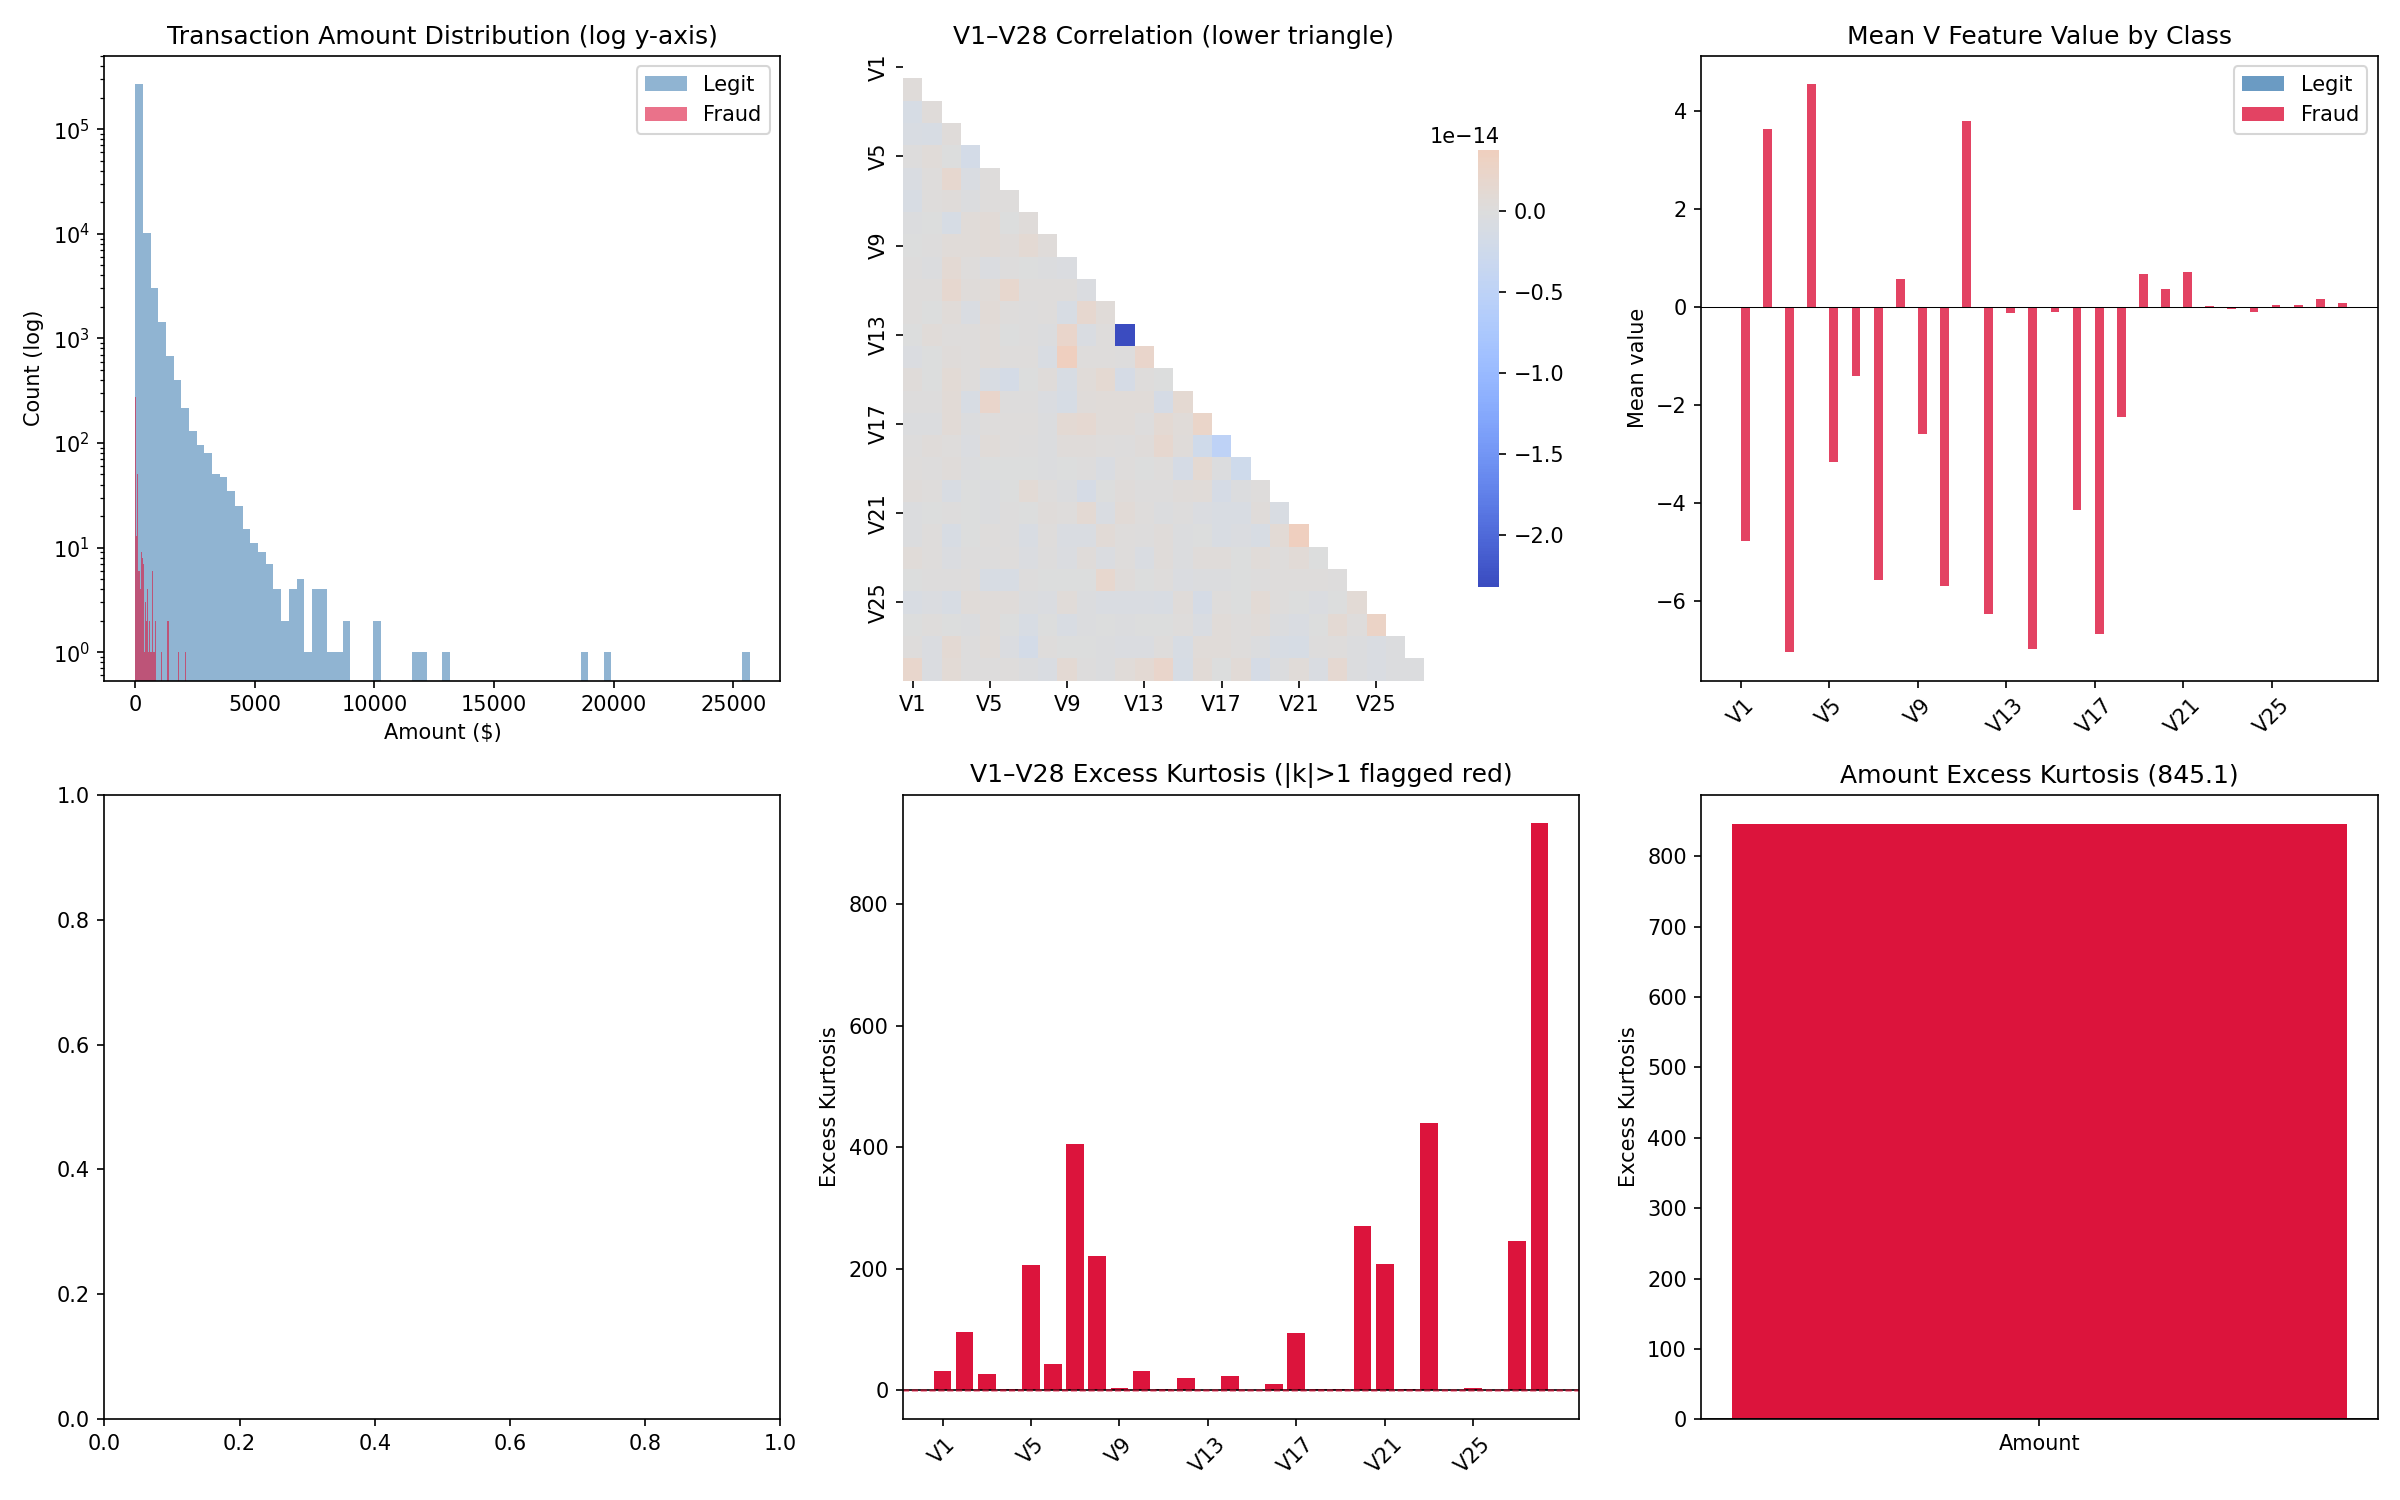
\includegraphics[width=\textwidth]{analysis.png}
\caption{Credit Card Fraud Detection -- transaction amount distribution, V1--V28 correlation structure, mean V-feature value by class, and excess kurtosis per feature (flagging the heavy-tailed PCA components discussed in the Datasets section).}
\label{fig:eda-cc}
\end{figure}

\subsection{Yahoo Webscope S5}

\begin{figure}[H]
\centering
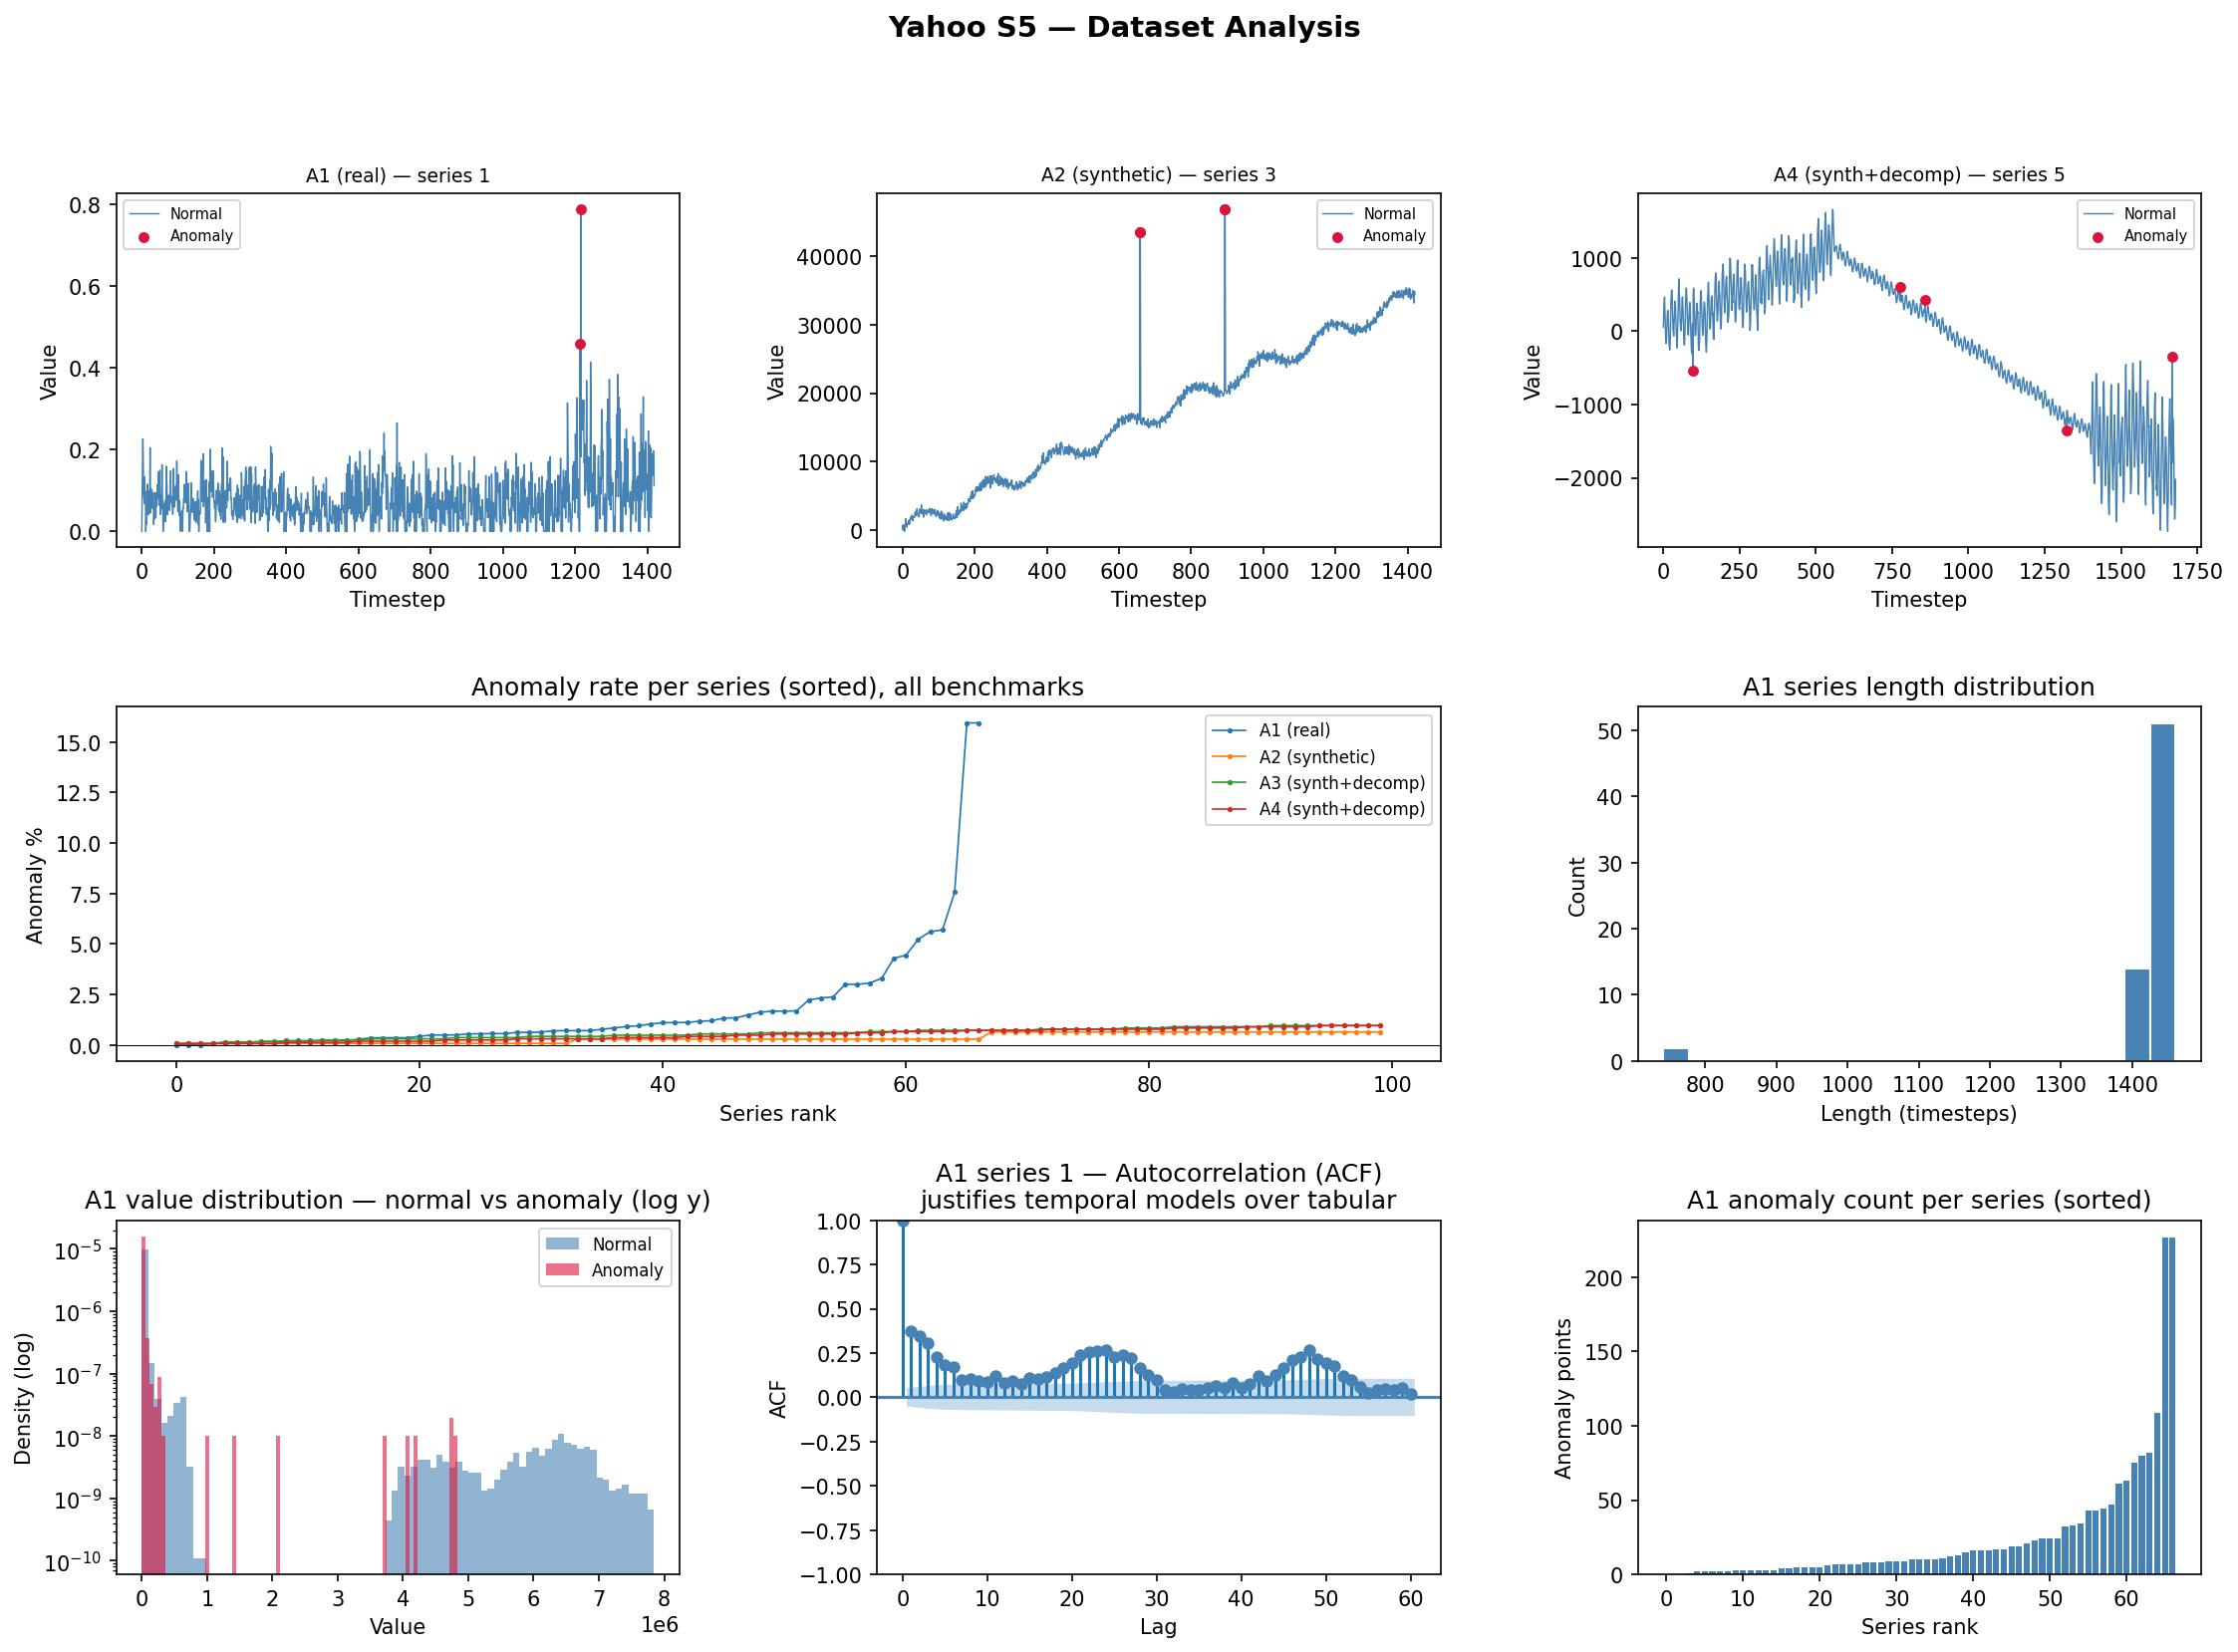
\includegraphics[width=\textwidth]{yahoo_analysis.png}
\caption{Yahoo S5 -- example series per benchmark, per-series anomaly rate, A1 series length distribution, A1 value distribution for normal vs.\ anomalous points, A1 autocorrelation (motivating the use of temporal models over tabular ones), and A1 anomaly count per series.}
\label{fig:eda-yahoo}
\end{figure}

\subsection{CIC-IDS2017}

\begin{figure}[H]
\centering
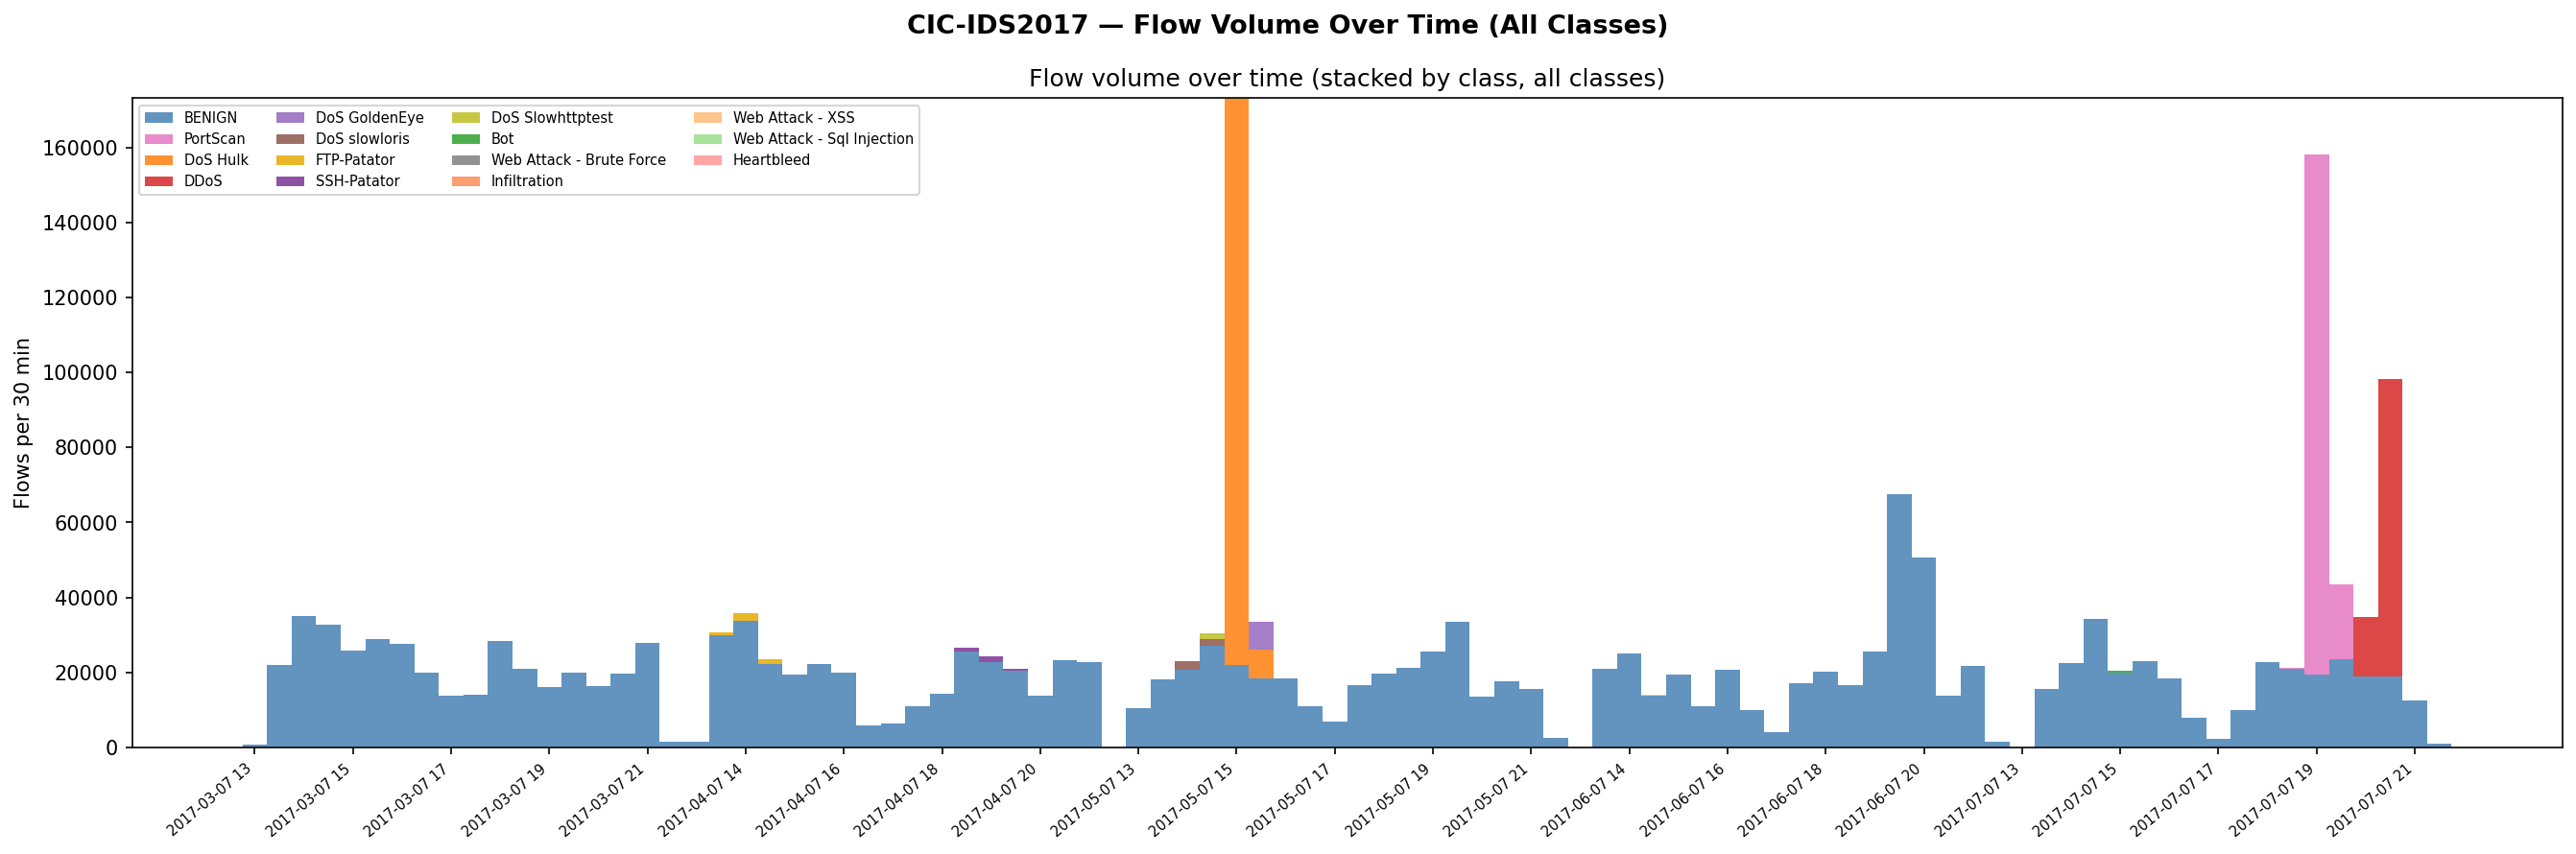
\includegraphics[width=\textwidth]{cicids_temporal_all.png}
\caption{CIC-IDS2017 -- flow volume over the capture week, stacked by class. BENIGN traffic dominates volume outside the concentrated attack windows visible on Tuesday--Friday.}
\label{fig:eda-cic-temporal-all}
\end{figure}

\begin{figure}[H]
\centering
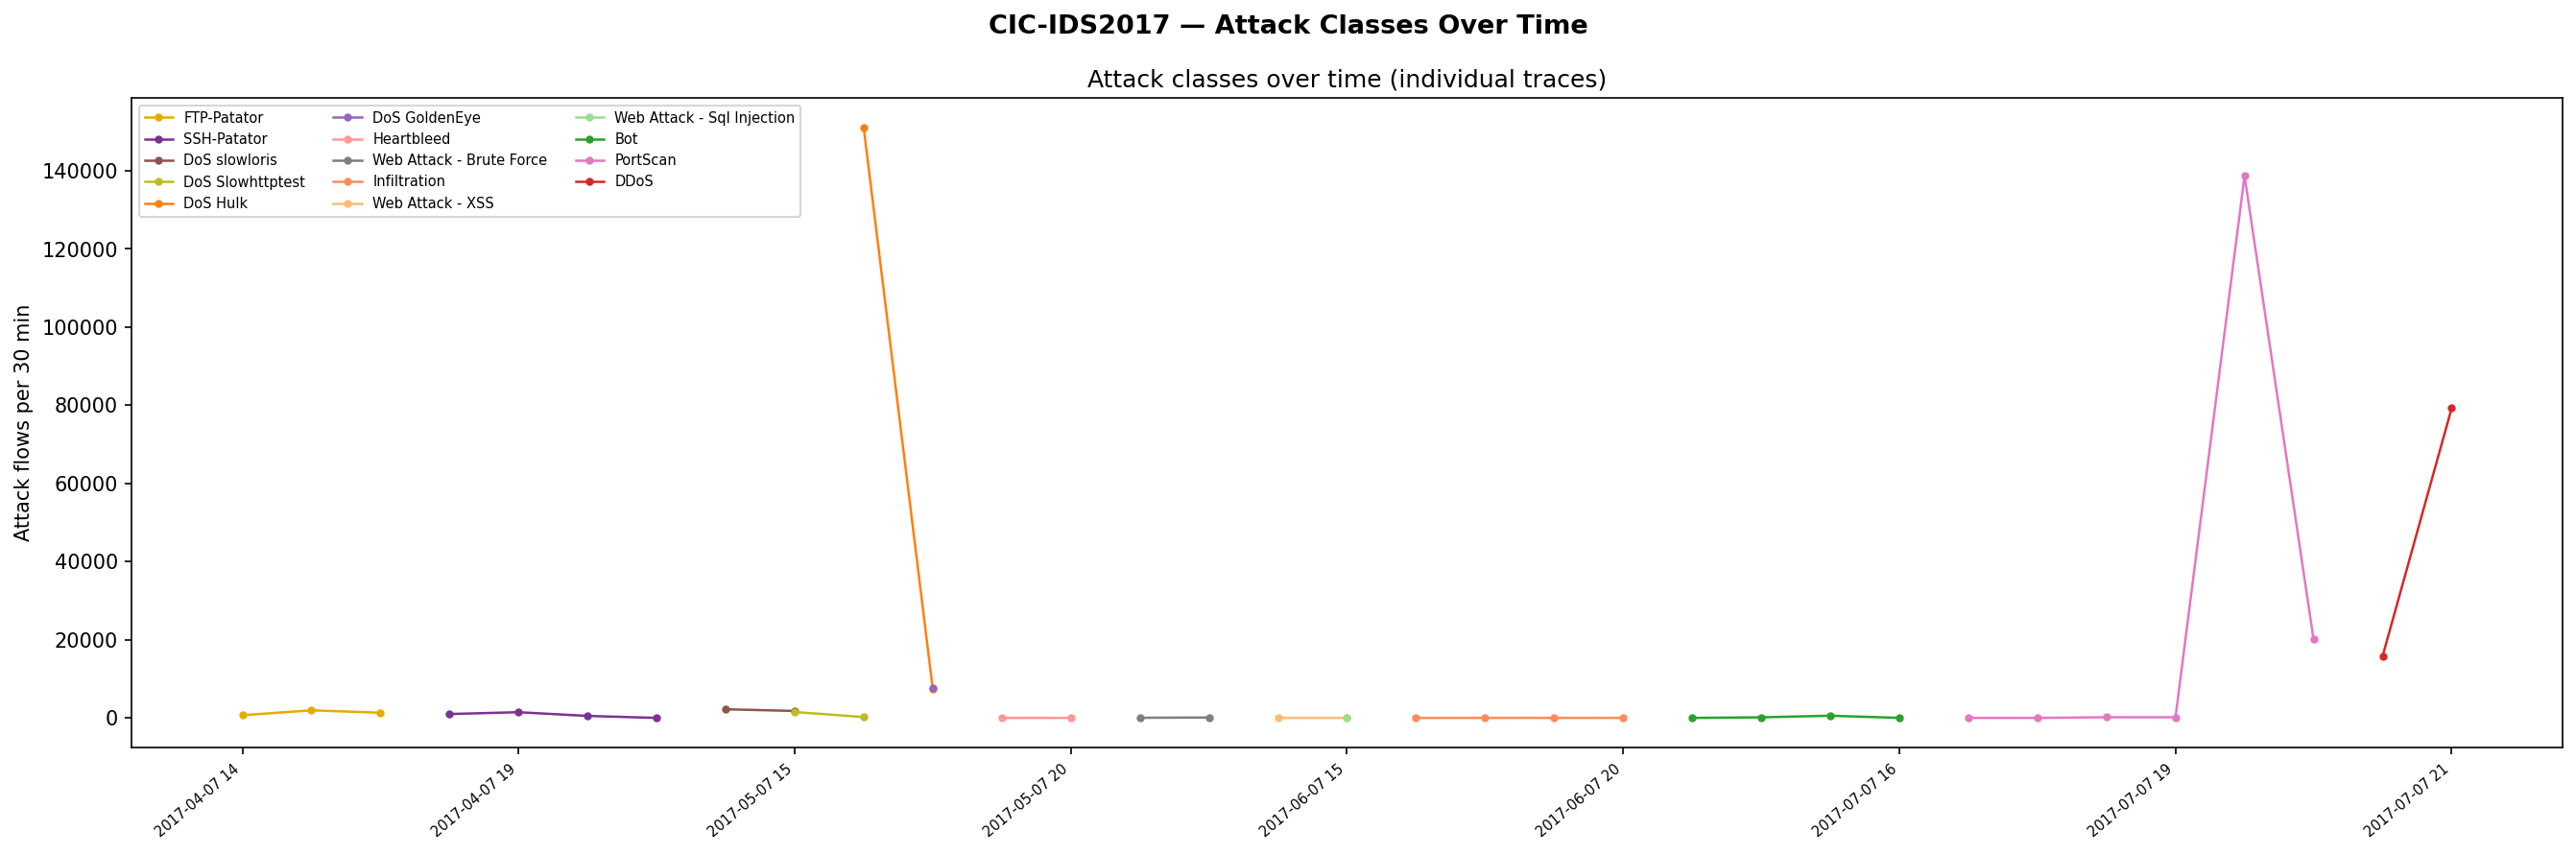
\includegraphics[width=\textwidth]{cicids_temporal_attacks.png}
\caption{CIC-IDS2017 -- attack classes over time, individual traces. Each attack occupies a short, distinct time window, confirming that attack classes do not overlap temporally within the capture.}
\label{fig:eda-cic-temporal-attacks}
\end{figure}

\begin{figure}[H]
\centering
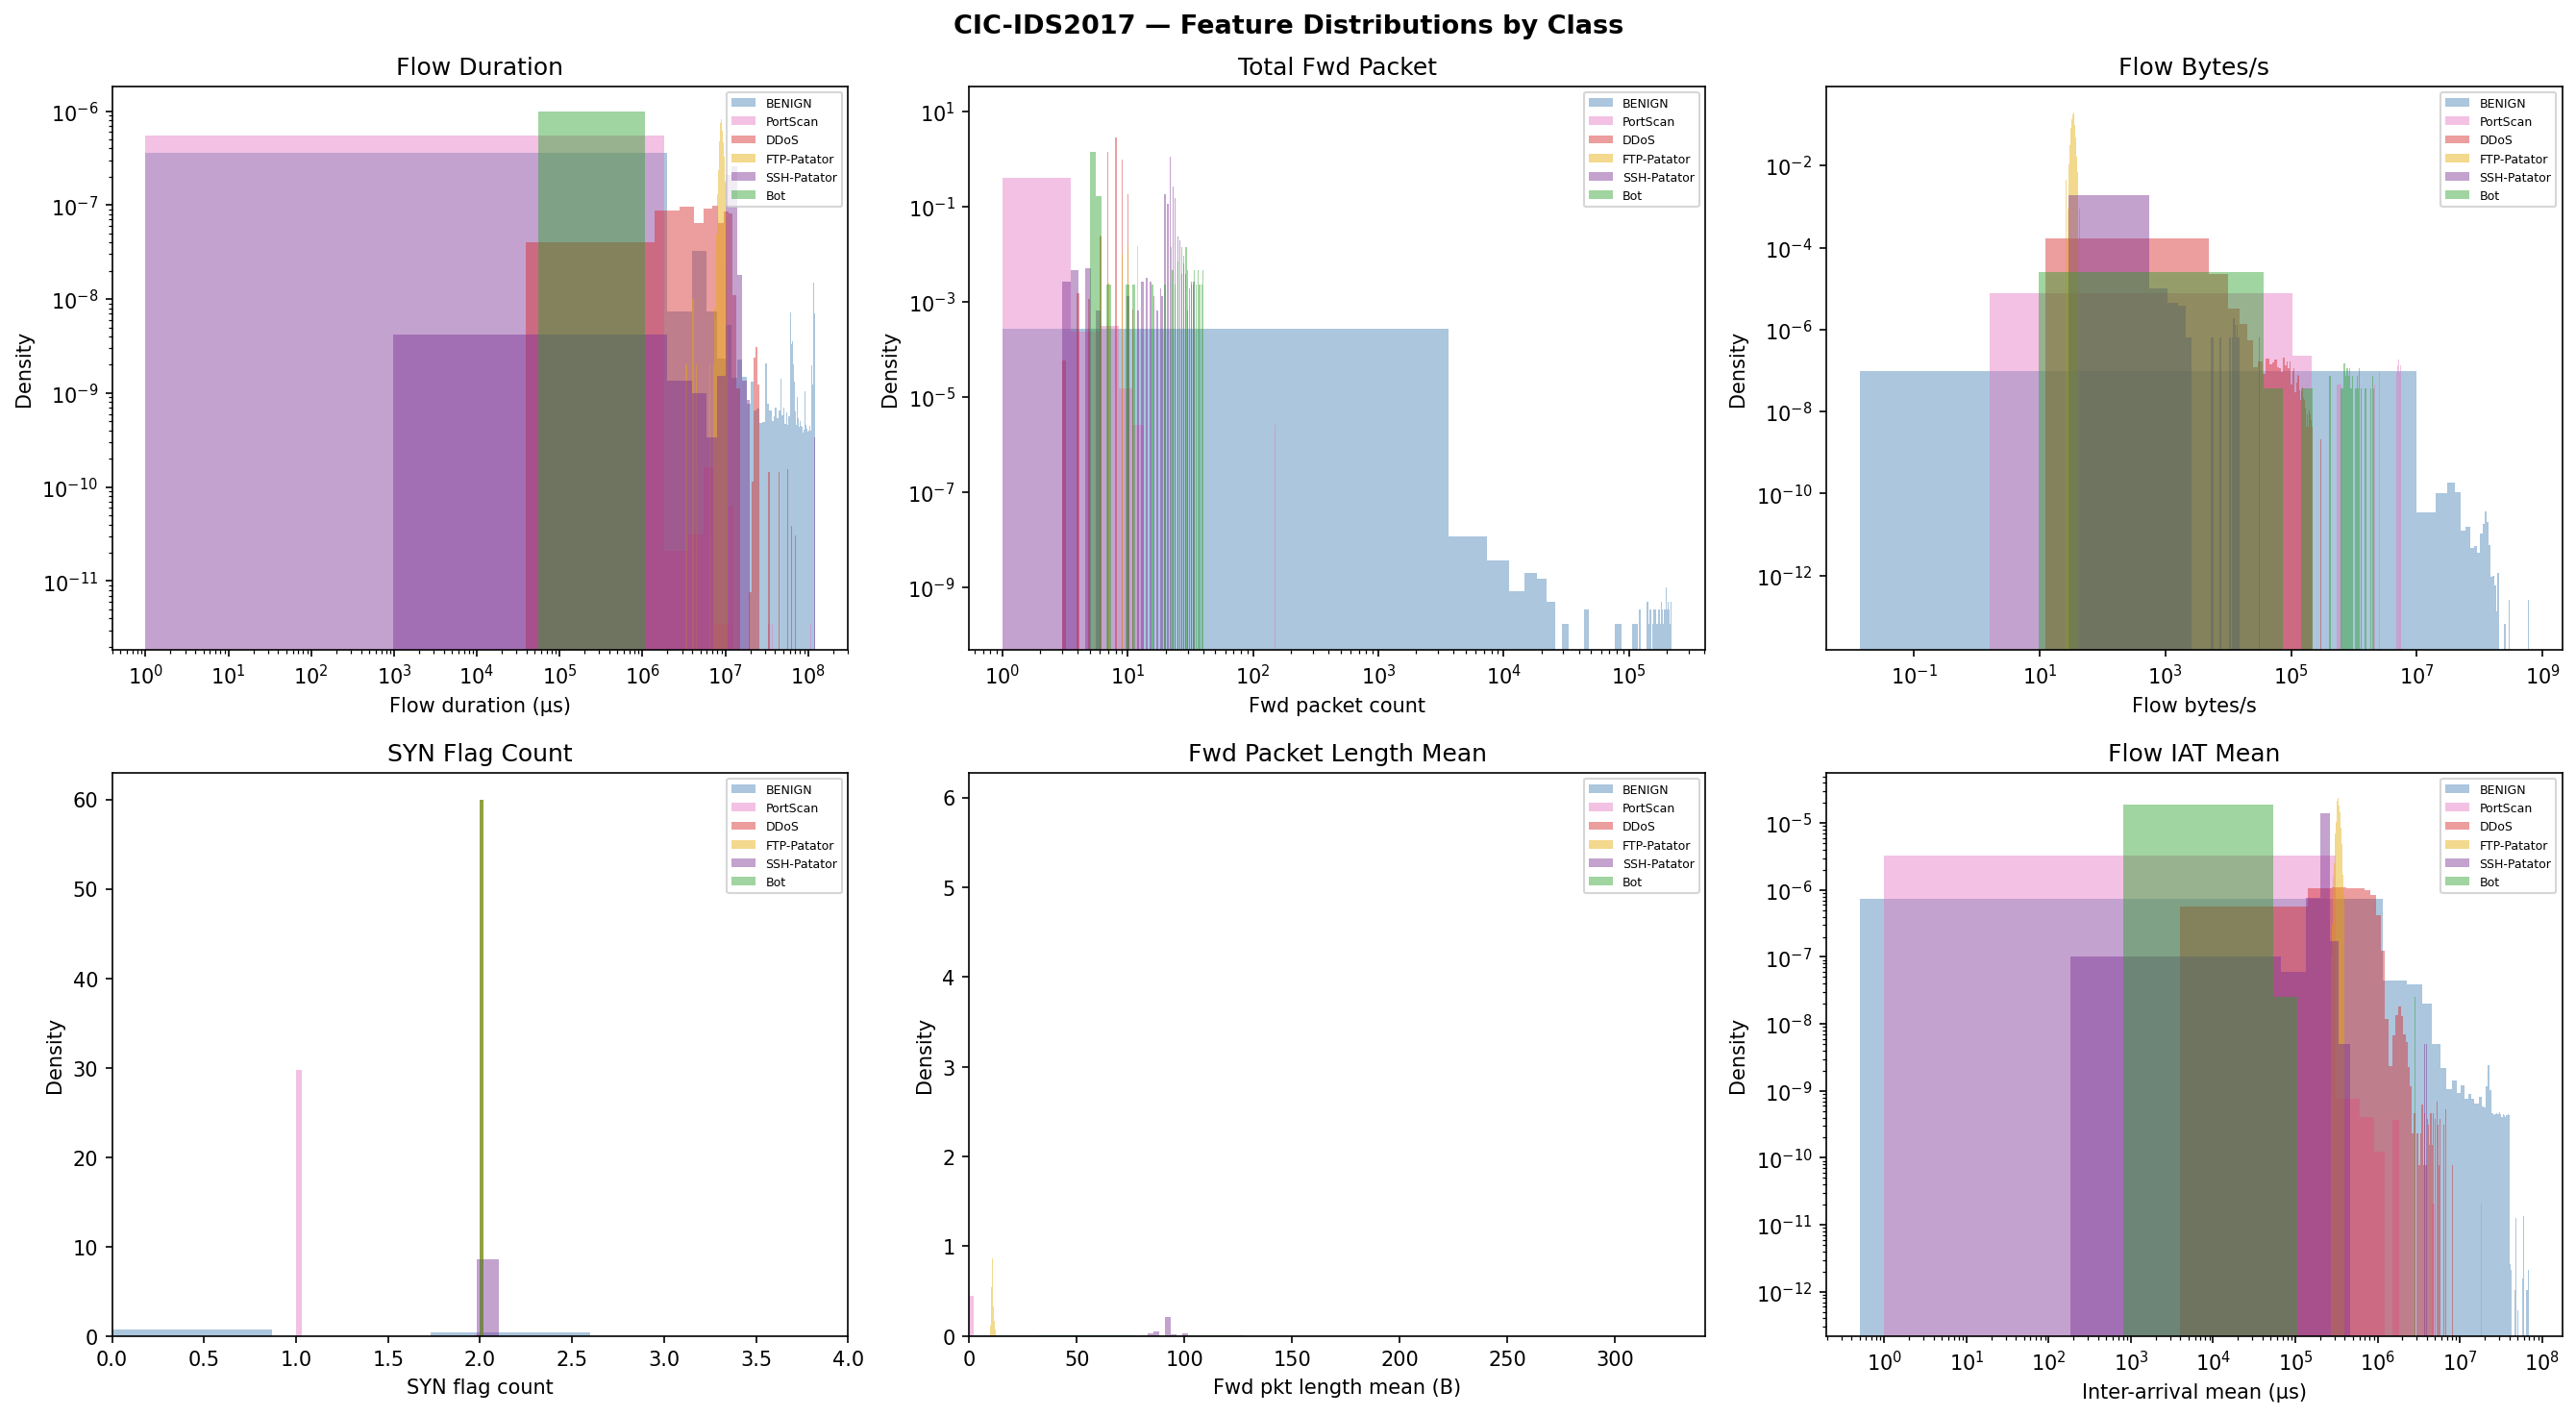
\includegraphics[width=\textwidth]{cicids_feature_profiles.png}
\caption{CIC-IDS2017 -- per-class distributions of six flow-level features (flow duration, forward packet count, flow bytes/s, SYN flag count, forward packet length mean, inter-arrival mean) for BENIGN and five representative attack classes.}
\label{fig:eda-cic-profiles}
\end{figure}

\section{Explainability}
\label{sec:explainability}

This section is a placeholder for the explainability analysis (SHAP attributions, reconstruction-error heatmaps, latent-space visualisation, and related diagnostics), to be filled in as that work is completed.

\printbibliography[heading=bibintoc]

\end{document}
